\title{
  %% IoTデバイスに電源と時刻と例外を提供する RaspberryCom*PoTE の設計実装
  %% %% と使われなくなった情報コンセントの活用事例
  IoTデバイスに電源と環境情報と例外発生を供給する方式とこれを用いた開発支援環境の提案\\
  ーRaspberry Com*PoTE を用いた Raspberry Workbench の設計と実装ー
}

\etitle{
  Design and Implementation of Raspberry Workbench to Supply IoT Devices Electrical  Power, Environmental Information, and Exceptions by using RaspberryCom*PoTE
}

\affiliate{Kanazawa}{金沢大学 学術メディア創成センター\\
Kakuma-machi, Kanazawa, Ishikawa 920-1192, Japan}
%% \affiliate{USP}{ユニバーサル・シェル・プログラミング研究所}

\author{大野 浩之}{Hiroyuki Ohno}{Kanazawa}[hohno@staff.kanazawa-u.ac.jp]

%% ---------------------------------------------------------
%% 概要(90%)(0.75p タイトルと概要)
%% ---------------------------------------------------------

\begin{abstract}
 一般に,IoTデバイスを運用するには,安定した電源供給が必要である.
 また,各IoTデバイスに正確な時刻を保持させたい場合が多い.
 さらに,多数のIoTデバイスを運用する場合には,特にその開発時や運用初期においては遠隔から指示で一斉再起動を行いたい場合が少なからずある.
 そこで,多数のIoTデバイスに対し,外部から「電源」「時刻等の情報(環境情報)」さらに「例外状態発生の通知」を安定して提供するしくみを設計し,これを {\tt Raspberry\-Com*PoTE}(ラズベリー・コンポート)と名付けた.
 本報では{\tt Raspberry\-Com*PoTE}の概要と,これを用いたIoTデバイス開発環境({\tt Raspberry\-Workbench}(ラスベリー・ワークベンチ))について報告する.


%% 一般に,IoTデバイスを長期間安定して運用するには,安定した電源供給が必要である.
%% また,著者が多数のIoTデバイスを運用する場合には,
%% 用途と状況にもよるが遠隔から強制的に一斉再起動を行いたい場合が多い.
%% さらに,各デバイスに正確な時刻を共有させたいことも多い.
%% そこで,IoTデバイスに対し,外部から電源と時刻と例外状態を安定して提供するしくみを設計し,これを {\tt RaspberryCom*PoTE}(ラズベリー・コンポート) と名付けた.
%% 本報告では,大学の研究室程度の規模の室内環境での運用を前提とした{\tt Raspberry\-Com*PoTE}の設計実装とその運用について報告する.
\end{abstract}

\begin{jkeyword}
IoT, ものづくり, ものグラミング, Raspberry Pi, Arduino, POSIX, POSIX中心主義, 有線IoT
\end{jkeyword}


\begin{eabstract}
Stable power supply is considered necessary for stable operation of IoT devices for a long period of time.
Depending on the application, it may also be necessary to enable a forced restart from a remote location.
In addition, when operating a large number of IoT devices, it may be necessary to supply an accurate time.
Therefore, we designed a system that provides power and time from outside to IoT devices and provides stable notification of exceptional conditions. We named it {\tt Raspberry\-Com*PoTE}.
In this report, we report on the design, implementation and operation of {\tt Raspberry\-Com*PoTE} on the premise of operating in an indoor environment of the size of a university laboratory.
 Furthermore, we also report on the IoT device development environment ({\tt Raspberry\-Workbench}) using {\tt Raspberry\-Com*PoTE}.

\end{eabstract}

\begin{ekeyword}
IoT, Mono-gramming, Monogramming, Raspberry Pi, Arduino, POSIX, POSIX centrics approach, Wired IoT
\end{ekeyword}

\maketitle


%% \underline{(ここまでで0.75p)}\\

%% ---------------------------------------------------------
%%  1. はじめに(00%)(0.25p / 1.0)
%% ---------------------------------------------------------

%% \section{はじめに \textcolor{red}{\small{\underline{(0.25p / 1.0)}}}}
\section{はじめに}
\label{sec:01introduction}

IoTデバイスを長期間に渡って安定運用するには,安定した電源供給が必要である.
このため,さまざまな方法が考案されている.
たとえば,IoTデバイスの消費電力を極力小さくした上で,「内蔵した電池が当該デバイスの想定運用期間中は寿命を迎えず給電を続ける」方法はその一つである.
この方法であれば,電源まわりは電池から給電のみを想定すればよく,電池交換のための機構や外部からの給電や充電方式については考える必要はなくなる.
しかし,この方法が利用できるIoTデバイスの消費電力は現状ではそれほど大きくはできない.
たとえば,
数時間に一度の頻度で,センサを使って得た計測結果を無線ネットワーク経由で母機となる機材に通知し,通知が終了したら直ちに深い休眠状態(以後「ディープスリープ」)に入るといった用途であれば,電池交換なしに数年間の連続運用を可能にした例がある.
一方,母機から予告なしに発せられる予定できない指示にしたがってアクチュエータを動かすといった用途では,外部からの給電あるいは電池交換なしに年単位の連続運用は現状では困難である.

このような例では,組み込み用のマイクロコントローラ(以後「組み込みマイコン」)を用いるのが普通であるが,近年広く普及している手のひらサイズのコンピュータである Raspberry Pi\cite{data:RaspberryPi} の場合は,アイドリング状態であっても 5V 300mA程度の電力を消費し,組み込みマイコンでは容易に実現できるディープスリープには入れない.このため,同機と同程度の大きさの IoTデバイス用としては比較的大きなバッテリーを組み合わせた場合でも,外部からの定期的な充電または常時給電なしに年単位運用を継続することはできない.

このような消費電流が大きい用途では,太陽電池等で必要な電力を独自に得て蓄電して自給する方法もあるが,十分な明るさを確保できない室内や夜間にも運用する用途には適さない場合がある.
最近では電場や磁場を介して電力を空間伝送する例もあるが,この方法も有効な場面は限られている.
結局,外部から有線によって電源を供給する従来の方法を必要とする場面は残っており,新たな技術的検討も意味がある.

上記の電源供給方法の議論とは別に,開発段階のIoTデバイス多数を最終的な設置形態を想定しつつ長期間に渡って無人連続運転を行うといった,開発工程の最終段階でには,当該IoTデバイス群のファームウェアを遠隔から更新したり,任意のタイミングで強制的に再起動するしくみがあると便利である.

さらに,多数のIoTデバイスを連携して運用する場合には,それぞれのIoTデバイスが正確な時刻を常に保持しているか必要に応じて取得できると,IoTデバイスの活動を記録する際に適切なタイムスタンプを付与できる.
IoTデバイスの規模が比較的大きければ,RTC(リアルタイムクロック)を搭載する方法があり,さらにIP接続性が確保できるなら,NTPプロトコルを始めとする時刻同期用のプロトコルを用いて
RTCを随時更新する方法が実用的であるが,小型のセンサと最小規模のマイコンの組み合わせなどでは仮に RTCの搭載は可能でも IP接続性の確保や NTPプロトコルの搭載が難しい場合がある.
このとき,RTCを搭載していても基準となる時刻と同期できなければ,タイムスタンプとしては役に立たない点に注意が必要である.
%%(※メモ:この文↑もう少し調整)

このような背景の下,大学の研究室程度の規模の室内環境での運用を前提に,
「IoTデバイスに
電源\textgt{\textbf{(\underline{Po}wer)}} と
時刻等の環境情報\textgt{\textbf{(\underline{T}ime)}}と
例外状態の発生\textgt{\textbf{(\underline{E}xception)}} を
外部から安定供給する
共通\textgt{\textbf{(\underline{Com}mon)}} の
複合的\textgt{\textbf{(\underline{Com}plex)}}な機構とそのための
構成要素\textgt{\textbf{(\underline{Com}ponent)}}
」を設計実装し,これを
%% \textgt{\textbf{Raspberry\underline{Com*PoTE}}}
{\tt Raspberry\underline{Com*PoTE}}
(ラズベリー・コンポート)と名付けて著者の周囲での供用を開始した.

さらに {\tt Raspberry\-Com*PoTE} を用いた IoT デバイス開発環境を試作し,これを
{\tt Raspberry\-Workbench}(ラズベリー・ワークベンチ)
と名付けた.

本報告では,{\tt Raspberry\-Com*PoTE} の設計と実装を述べ,
および {\tt Raspberry\-Workbench} についても言及する.


%% ---------------------------------------------------------
%%  2. 背景(00%)0.75P / 1.75
%% ---------------------------------------------------------
%% \section{背景 \textcolor{red}{\small{\underline{(0.75p / 1.75)}}}}
\section{背景}
\label{sec:02background}

本研究では,大学の研究室のような規模の室内環境でIoTデバイスを長期に渡って安全安心かつ簡単に取り扱える環境の整備に主眼を置く.

これまでも著者は,RaspberryGateや RaspberryGuardianを設計実装して,IoTデバイスへの不適切なアクセスを防御するためのセキュリティゲートウェイの構築と運用機構を実装したり\cite{hohno:RaspberryGate}\cite{hohno:RaspberryGuardian} ,
I2Cベースの近距離有線ネットワークを提案して室内環境でのIoTデバイスの運用環境を提供したり\cite{hohno:I2CwiredLAN-2017},
「ものグラミング」と名付けたIoT環境向けプログラミング手法を提案したりしてきた\cite{hohno:monogramming2}.

今回は,著者が 2017年に Raspberry Leaves として報告した「I2Cベースの近距離有線IoTネットワーク」の運用経験を踏まえ,これを一部を簡素化した上で新たな機能を追加したしくみを検討した.
具体的には,2017年に提案した方式(以後「2017年方式」)から長距離I2C通信機能を削除し,これに伴いI2Cバスから基準信号を抽出する機能も削除した.
代わりに以下の機能を改良あるいは追加し,簡単で使い勝手のよいしくみの実現を目指した.
%% なお,2017年に報告したI2Cベースの近距離有線ネットワークには特段の名前がついていないので,以後「2017年方式」と呼ぶ.

\begin{itemize}
\item (改良) 安定した電源供給
\item (強化) 例外状態(ハードウェア・リセット,ハードウェア割り込み)の通知
\item (新規) 環境情報(時刻等・後述)の通知
\end{itemize}

長距離I2C通信機能は,2017年方式には存在したものの本研究では削除したが,信号伝送方式を差動型に変更して通信距離の延長と安定を確保した差動型I2C通信方式は現在評価中である.
この成果は次世代の {\tt Raspberry\-Com*PoTE} に取り込む方針である.
%%% ※ これについては考察で言及する.

%% (※メモ:↑「考察で言及」してね)

%% (※メモ) これまでIOT環境関連では以下を実施してきた\\
%% \begin{itemize}
%% \item Raspbery Gate
%% \item Raspbery Guardian
%% \item ものぐらみんぐ
%% \item I2Cベースの近距離有線ネットワーク(2017年方式)
%% \end{itemize}

%% (※メモ) 前提となる現在の(自分の)研究環境\\

%% (※メモ) 現状,少なくとも現用の環境では室内に設置されたIOTデバイスには以下の需要がある\\
%% \begin{itemize}
%% \item (必須)安定した電源供給
%% \item (重要)例外状態通知(再起動, H/W割り込み)
%% \item (有用)時刻等の環境情報の通知
%% \end{itemize}

%% ---------------------------------------------------------
%%  3.関連研究(00%)0.75P / 2.5
%% ---------------------------------------------------------
%% \section{関連研究 \textcolor{red}{\textcolor{red}{\small{\underline{(0.75p / 2.5)}}}}}
\section{関連研究}
%% \vspace{-0.5zh}
\label{sec:03relatedworks}

\subsection{2017年方式(Raspberry Leaves)}
%% \vspace{-0.5zh}

本研究で提案する{\tt Raspberry\-Com*PoTE}に最も近いのは,著者が取り組んだ2017年方式である.
{\tt Raspberry\-Com*PoTE}は2017年方式の延長上にある.

2017年方式では8芯ケーブルの使用を前提とし,そのうちの4芯で電源と有線通信機能(実体は駆動電圧を12Vに上げて通信距離の延長を実現したI2Cバス互換の通信方式)を提供し,残りの4芯を2つ目のI2Cバスにしたり,1-Wire を使った構成管理機能に割り当てたりした.
2017年方式を{\tt Raspberry\-Com*PoTE}と比べると,電源を供給するという考え方は同じであるが,{\tt Raspberry\-Com*PoTE}ではI2Cバスベースの双方向有線通信は提供していないし,
I2Cバスを持たないため,I2Cバスのロックアップ回避・回復機能も持たない.
一方,{\tt Raspberry\-Com*PoTE}は有線通信のためRS-485を採用しているので低速な双方向通信は可能である.しかし,現時点では以下で述べる「環境情報」を提供するためだけに用いており,結果的に一方向通信になっている.

両方式ともIoTデバイスに時刻情報を供給することは重要だと考えているが,2017年方式では基準時間信号と称する正確なクロックを提供しようとしているのに対して,{\tt Raspberry\-Com*PoTE}では時刻そのものを適切なタイミングで供給している.
また,{\tt Raspberry\-Com*PoTE}では時刻を「環境情報」の一つと位置づけており,時刻以外にもIoTデバイス群が設置された環境に関する諸情報(気温,湿度,気圧,明るさ等)を供給・共有できる.
さらに,{\tt Raspberry\-Com*PoTE}では必須の機能として実現しているハードウェア割り込みやハードウェア・リセットは,2017年方式ではオプション機能と位置づけ,1-Wireを使った構成管理機能に委ねているため必須機能ではなかった.

以上をまとめたのが表\ref{tb:T2017_vs_RaspberryComPoTE}である.
{\tt Raspberry\-Com*PoTE}は2017年方式の開発経験を踏まえているが採用しなかった機能もあるため完全な後継ではない.

%% \vspace{-0.5zh}
\begin{table}[h]
  \centering
  \begin{tabular}{|l|c|c|l|} \hline
    機能 & 2017年方式 & ComPoTE &  備 考 \\
    \hline
    電源供給 & \checkmark & \checkmark &\\
    有線通信 & \checkmark {\tiny (I2C)} & \checkmark {\tiny (RS-485)} &\\
    基準クロック & \checkmark & − &\\
    現在時刻 & − & \checkmark &\\
    環境情報 & − & \checkmark & {\tiny 時刻以外は準備中}\\
    構成管理 & \checkmark {\tiny (1-Wire)} & − & {\tiny オプション}\\
    割り込み & − & \checkmark &\\
    リセット & − & \checkmark &\\
    \hline
  \end{tabular}
  \label{tb:T2017_vs_RaspberryComPoTE}
  \caption{2017方式と{\tt Raspberry\-Com*PoTE}の比較 (\checkmark が該当ありを示す)}
\end{table}
%% \vspace{-1.0zh}

%% (※メモ:↑続き書いてね!← OK※)

\subsection{有線IoT}
%% \vspace{-0.5zh}

{\tt Raspberry\-Com*PoTE} は「有線IoT」と呼ばれる分野に属する.
この分野では,既存のイーサネット技術を元に最長1kmの距離で最大10Mbpsのデータ伝送速度と1〜50Wの給電を1組の撚対線で実現する,シングルペアイーサネット(10BASE-T1L, IEEE802.3cg)が2020年に標準化されており,主たる用途は車載機器や産業機器とされており,小規模な室内環境での利用を視野に入れている\cite{misc:802.3cg}.
%% 標準化後には大いに注目される技術になると予想できるが,現時点では当該規格に準拠した製品を入手できる状況ではない.
著者の 2017年方式も{\tt Raspberry\-Com*PoTE}も室内のような小規模な領域での利用を前提としている.
%% どちらも数10m程度の利用を想定している.
{\tt Raspberry\-Com*PoTE}には通信機能が搭載されておらず,通信が必要な場合には WiFi や Bluetooth などの通信方式を併用する必要があるし,電力供給のための電源電圧も12〜15V程度であり,IEEE802.3cgが50Wを供給するためにDC60Vを想定していることと比べると{\tt Raspberry\-Com*PoTE}が適用できる用途や範囲はIEEE802.3cgの適用範囲より小規模になる.
なお,{\tt Raspberry\-Com*PoTE}には環境情報の提供や例外状態の通知など IEEE802.3cg にはない機能を有しているため,この機能を必要とする用途であれば{\tt Raspberry\-Com*PoTE}に優位性がある.

%% https://www.analog.com/en/technical-articles/the-new-10base-t1l-standard.html

%% https://businessnetwork.jp/Detail/tabid/65/artid/6561/Default.aspx

%% (※メモ:↑続き書いてね!← OK※)

\subsection{PoE}
%% \vspace{-0.5zh}

通信用の配線を使い,通信しつつ電力を供給する方式としては PoE(PowerOverEthernet)が普及している.
PoEの基本機能は2003年に発効したIEEE 802.3afで規定されており,これに従えばカテゴリ5以上のUTPケーブルを使って電力を供給できる.
通常,電力送出側の機器は直流48V前後で送電し,受電側は最大で約13Wの電力を取り出せる.
PoEは,有線環境で電力供給と通信を両立させる方式としてはもっとも成功している.
{\tt Raspberry\-Com*PoTE}をPoEと比較すると,通信機能も電力供給も劣るが,PoEにはない環境情報の提供や例外状態の通知などの特定目的に特化した機能を有する.
また,電力供給のためにPoEが利用する48V前後の電圧は電子回路の開発者にとっては高圧であり,開発中の接触事故や短絡事故などの際に周辺に与える損傷は,15V前後の
電圧を用いる{\tt Raspberry\-Com*PoTE}の場合より大きい.

%% (※メモ:↑続き書いてね!)

\subsection{PLC}
%% \vspace{-0.5zh}

PoEとは逆に,交流電力線を使って電力を供給しつつ通信を重畳する方に PLC(PowerLineCommunication 電力線通信)がある.

%% https://www.ntt.co.jp/journal/0407/files/jn200407088.pdf

日本においては周波数の低い 50Hzや60Hzの交流電力線に450kHz以下の帯域の信号を重畳して通信を行う方式がまず実用化され,
その後 2006年には 2〜30MHzの帯域も利用できるようになった.
後者は高速電力線通信と呼んで前者と区別する場合がある.前者では9600bps程度,後者では100Mbpsを超える通信速度を提供する機器が実用化されている.

一方,{\tt Raspberry\-Com*PoTE}ではハードウェア割込信号やハードウェア・リセット信号を直流の電源線に重畳するが,
その信号は数Hzあるいはそれ以下の速度で電源電圧を変動させることで実現している.すなわち供給する電力は直流である.
PLC技術は交流電力線に信号を重畳しているため,参考にはなる点もあるが {\tt Raspberry\-Com*PoTE} とは異なる方式である.


\subsection{DCC}
%% \vspace{-0.5zh}

%%% PLCではないが,


PoEでは,送信側は通信用の交流信号に電力用の直流を加えて送り,受信側では本来の信号と電力供給用の直流を分離して用いている.

PLC は,送信側は電力供給用の交流電力線に通信のための高周波信号を乗せて送り出し,受信側は交流電力を受電しつつ,重畳した高周波を取り出して複合し,受信した情報を得る方式である.
すなわち周波数の低い交流電力線に周波数の高い交流信号を重畳している.

これらに対して,送信側は送出したい情報を PWM 変調してこれをある程度の振幅の交流として送り出すことで,信号そのものに電力搬送の役割も担わせ,受信側は受け取った受け取った信号を復調して情報を得るとともに,これを整流することで電力とする方法も考えられる.
この,信号線に電力搬送も担わせる方式の一つに,鉄道模型の分野で模型の機関車をデジタル信号で遠隔操作する目的で使われている DCC (Digital Command Control) がある\cite{misc:DCC}.

DCCでは,制御装置から 2本のレールに ±12V 程度の振幅を持つ 数kHzのPWM信号を流しており,レール上の模型はこれを復調することで制御装置からの指令を受け取り,整流することで電力を得ることができる.DCCは,想定する運用環境の大きさも,運用に供する機材の数も,{\tt Raspberry\-Com*PoTE} が想定する環境に近い.
このため DCC を利用することも検討した.DCC にはすでに商用化されているという魅力があったが,{\tt Raspberry\-Com*PoTE}は I2Cバスをベースとする2017方式との統合も視野に入れているため,現時点での DCCの採用は見送った.
%% 差動通信方式を導入するとはいえ基本は 


%% (※メモ:↑続き書いてね!)

%% (※メモ) \\
%% \begin{itemize}
%% \item I2Cベースの近距離有線ネットワーク(2017年方式)
%% \item 有線IoT...
%% \item PoE...
%% \item PLC...
%% \item DCC...
%% \end{itemize}

%% ---------------------------------------------------------
%%  4. 設計と実装(00%)3P / 5.5
%% ---------------------------------------------------------
%% \section{設計と実装 \textcolor{red}{\small{\underline{(3.0p / 5.5)}}}}
\section{{\tt Raspberry\-Com*PoTE}の設計と実装}
%% \vspace{-0.5zh}
\label{sec:04design_and_implementation}

本節では,{\tt Raspberry\-Com*PoTE}の設計方針を明らかにし,さらに実際の設計と実装について述べる.

%% ---------------------------------------------------------

\subsection{方針}
%% \vspace{-0.5zh}

「電源供給」「環境情報提供」「例外状態通知」の3つの需要を満たす方法を設計実装するにあたり,以下の方針をとった.
なお,現時点では環境情報として提供しているのは時刻のみであるが,他の環境情報を提供することに技術的困難はない.

\begin{enumerate}
\item (配線)配線に用いる線数(配線材の芯数)はできるだけ少なくするなど,全体として簡素であることを重視する
\item (互換性)既存の類似の諸方式との互換性確保には固執しない
\item (通信)IoTデバイス同士や,IoTデバイスの母艦となる計測制御用コンピュータとIoTデバイスとの間で発生する実際の通信については積極的には提供しない
\item (開発速度)開発の初期段階から日常の研究開発環境に投入して常時利用し,問題点があれば直ちにフィードバックして改善・変更する方式を採用し開発速度を上げる
\end{enumerate}

%% (※メモ:↑もう少し書けない?)

これらのうち第3項については,
後述するように{\tt Raspberry\-Com*PoTE} では,環境情報の提供に RS-485 による有線通信を用いているので,{\tt Raspberry\-Com*PoTE} が提供する機能を用いて IoTデバイス同士やIoTデバイスと計測制御用コンピュータが相互に通信することは可能である.
しかし,このような機材間の通信は,頻度,通信量,実時間性への要求などが利用形態によって全く異なる.このため,RS-485 で対応可能か否かは利用形態ごとに個別に検討する必要がある.
また,利用目的や利用形態が異なる複数の装置が一つの {\tt Raspberry\-Com*PoTE}を利用して電源や環境情報の供給を受けることは可能であるが,目的も形態も異なる装置が一つの RS-485ネットワークを利用すると回線の利用を調停する必要が生じ,簡素に実現することはできない.
一方,現在では機材間の通信は RS-485 より高速な WiFi, Bluetooth, その他の方法で実現できるのが普通であり,無理にRS-485の利用を強制する必要はない.そこで,機材間の実際の通信は {\tt Raspberry\-Com*PoTE} に含めないことにした.

この方針の下,{\tt Raspberry\-Com*PoTE} では4芯ケーブルを用いることとし,このうち2本で電源供給と例外状態通知を,残りの2本で環境情報の提供を実現することとした

ところで,2017年方式では8芯ケーブルを使うことを前提としている.
この8芯ケーブルを,今回提案する {\tt Raspberry\-Com*PoTE} で改めて利用すると4芯が残る.
この残った4芯を用いれば,2017年方式の実装後に別途実装と評価を行った「差動方式のI2Cバス」(4芯必要)を導入できる.
機材間の通信を含めて全てを有線で構成したい場合は,通信速度がI2C通信の速度に拘束されてしまう問題があるが,この差動方式のI2Cバスの採用が有力である.
すなわち,8芯ケーブルを用いれば,2017年方式が提供していた有線通信と {\tt Raspberry\-Com*PoTE}とを融合させた新たなあるいは拡張した方法を検討する余地がある.
このことについては今後継続的に検討を行う.

%% (※メモ:↑ちゃんと言及してね!)

%% ---------------------------------------------------------

\subsection{設計と実装}
%% \vspace{-0.5zh}

上述の方針に基づいて設計実装した {\tt Raspberry\-Com*PoTE} は以下の3つの系から構成される.

\begin{itemize}
\item 電源供給系
\item 例外状態通知系(送出系・検出系)
\item 環境情報提供系
\end{itemize}

上述の方針に基づいて設計実装した {\tt Raspberry\-Com*PoTE} の概要を図\ref{RaspberryComPoTE-X}に示す.
 {\tt Raspberry\-Com*PoTE}は +V, D+, D-, GND の 4線からなるバス型で,物理層は電源周りを強化し電力供給も可能にした RS-485 とみなせる.

\vspace{-1zh}
\begin{figure}[H]
\centering
%% 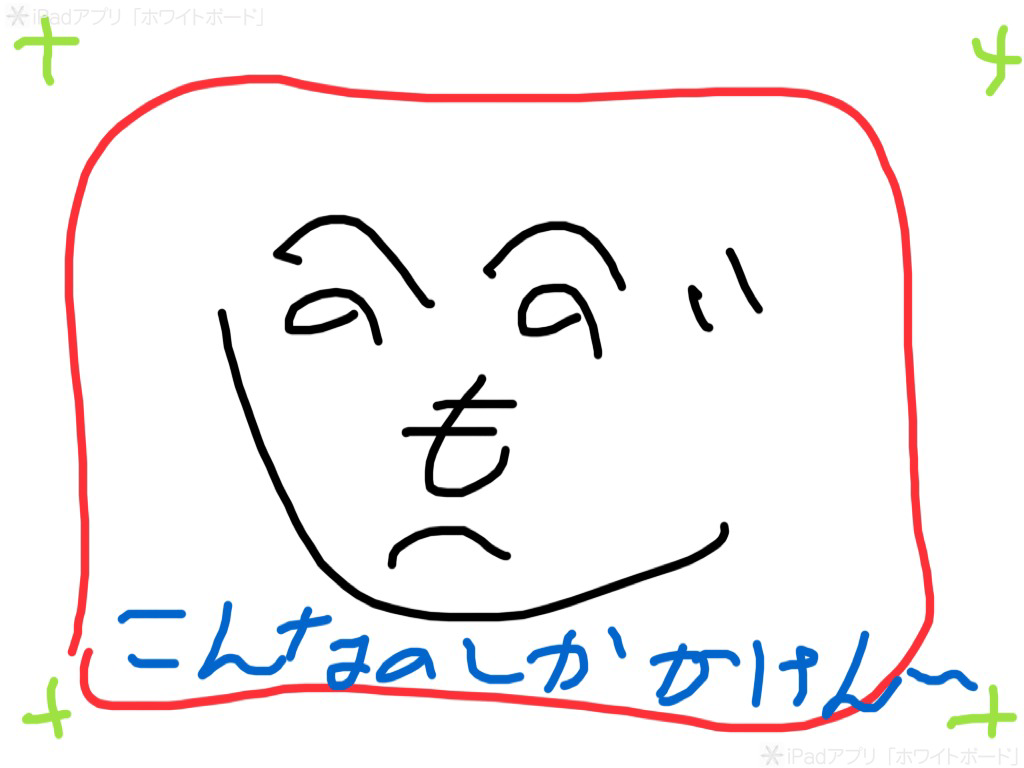
\includegraphics[width=5cm]{figspics/henoheno.png}

\includegraphics[width=8cm]{figspics/RaspberryComPoTE_figX2.png}
\caption{{RaspberryComPoTE}全体構成図}
\label{RaspberryComPoTE-X}
\end{figure}
\vspace{-1zh}

%% (※メモ:図)ここに全体構成図(図\ref{RaspberryComPoTE})を入れる
%%x%%
以下では上図に記された3つの系,すなわち電源供給系,例外状態通知系(送出系+検出系),環境情報提供系の設計と実装について述べる.
%%x%%

\subsubsection{電源供給系+例外状態送出系}
%% \vspace{-0.5zh}


電源供給系は,単なる定電圧電源ではなく二つの異なる電圧間を必要なタイミングで遅延なくおよそ0.1ないし2Hz程度の速度で遷移する機能を持つ.
これは,{\tt Raspberry\-Com*PoTE}では,例外状態の発生を電源電圧の変動で表現するためである.
%% 次項で述べるように
2017年方式にも存在するこの電圧繊維機能を伴う電源供給機能は,2017年方式と同様に「非安定電源機能」と呼んでいる.
非安定電源機能は,安定化電源装置の出力電圧を外部から意図的に変動させる.
この電位の変動は,受電側({\tt Raspberry\-Com*PoTE}を利用する各IoTデバイス側.図\ref{RaspberryComPoTE-X}にあっては IoTデバイス 01..NN)においては,
4芯ケーブルを経由することで生じる電圧降下も加わって相応に低下した状態となるが,重要なのは二つの状態に対応した電位そのものではなくその電位差である.
この電位差はほとんどの利用形態で送電側と受電側とでほぼ同じになる
\footnote{高電位状態での供給電流を $\text{I}_\text{H}$ ,
  低電位状態での供給電流を $\text{I}_\text{L}$ ,
  線路の直流抵抗をRとすると,受電側の電位差は厳密には
  $ \text{R} \times (\text{I}_\text{H} - \text{I}_\text{L}) $
  だけ小さくなるが,この差は今回の用途にとっては十分に小さい}.

なお,各機器が最終的に必要とする電源は,各機器ごとに用意する昇降圧型の電圧レギュレータで供給電圧を調整するため,
送出時点での電源電圧の変動と4芯ケーブルを経由することで発生する電圧降下の影響は,個別のIoTデバイスには及ばない.

現在の実装では,電源供給系自体への入力電圧は直流16V,出力電圧(送出電圧)は通常時が DC 13.5V前後,例外状態通知状態では 9V前後 としている.また,各IoTデバイスに搭載している昇降圧型電圧レギュレータの入力電圧は 4.5〜18V である.このため例外状態通知のため供給電圧が大きく低下しても最終的にIoTデバイスに供給される電圧は 5V(または 3.3V)を維持できる.

例外状態通知のための電源電圧の変動速度は 0.1〜2Hz程度なのでデータ通信としては超低速な部類になるが,
定電圧電源装置にスイッチングレギュレータを採用すると数Hzの速度であっても電圧を任意のタイミングで素早く変化させることは難しい.
これはスイッチングレギュレータでは,二次側に容量の大きなコンデンサを取り付けるのが普通で,この容量により出力電圧の設定を変更しても追従するのに秒単位の時間がかかるためである.
そこで今回は,スイッチングレギュレータより変換効率は劣るが,設定電圧の変化への追随が速いシリーズ型の定電圧電源回路を採用し,LM338 5A可変レギュレータ\cite{data:LM338}を用いて実装した.


現時点での電源供給と例外状態の送出を担う系の実装を図\ref{hohno:RaspberryComPoTE-Po1}に示す.\\
%%x%%
\vspace{-1zh}
\begin{figure}[H]
\centering
%%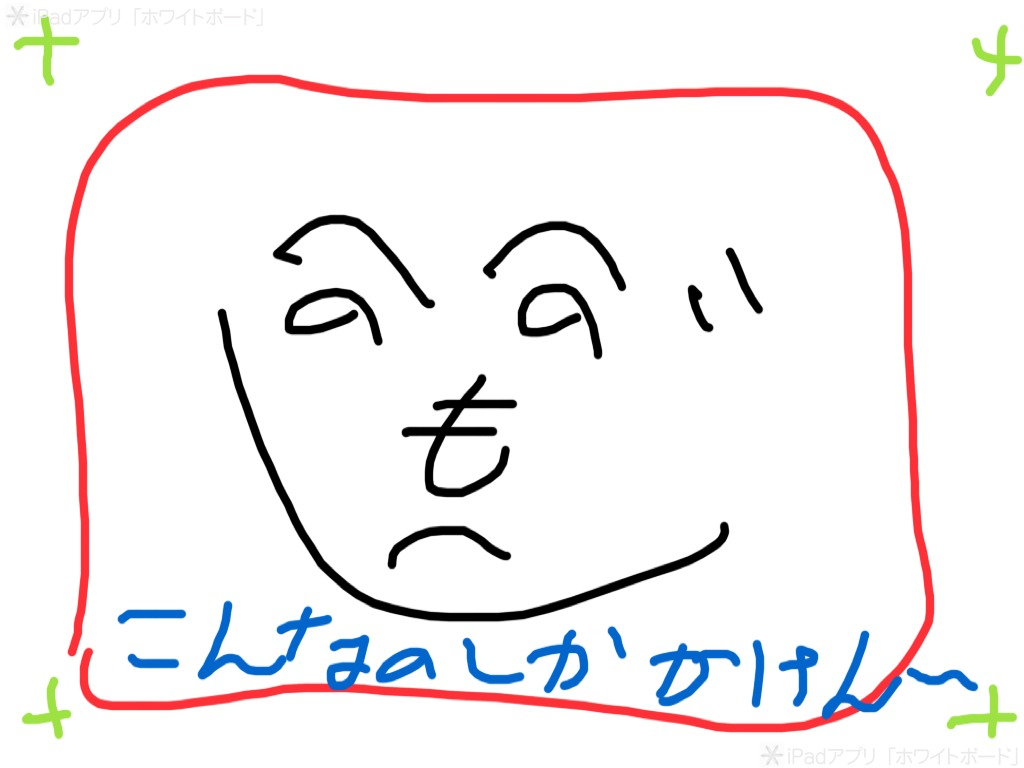
\includegraphics[width=5cm]{figspics/henoheno.jpeg}
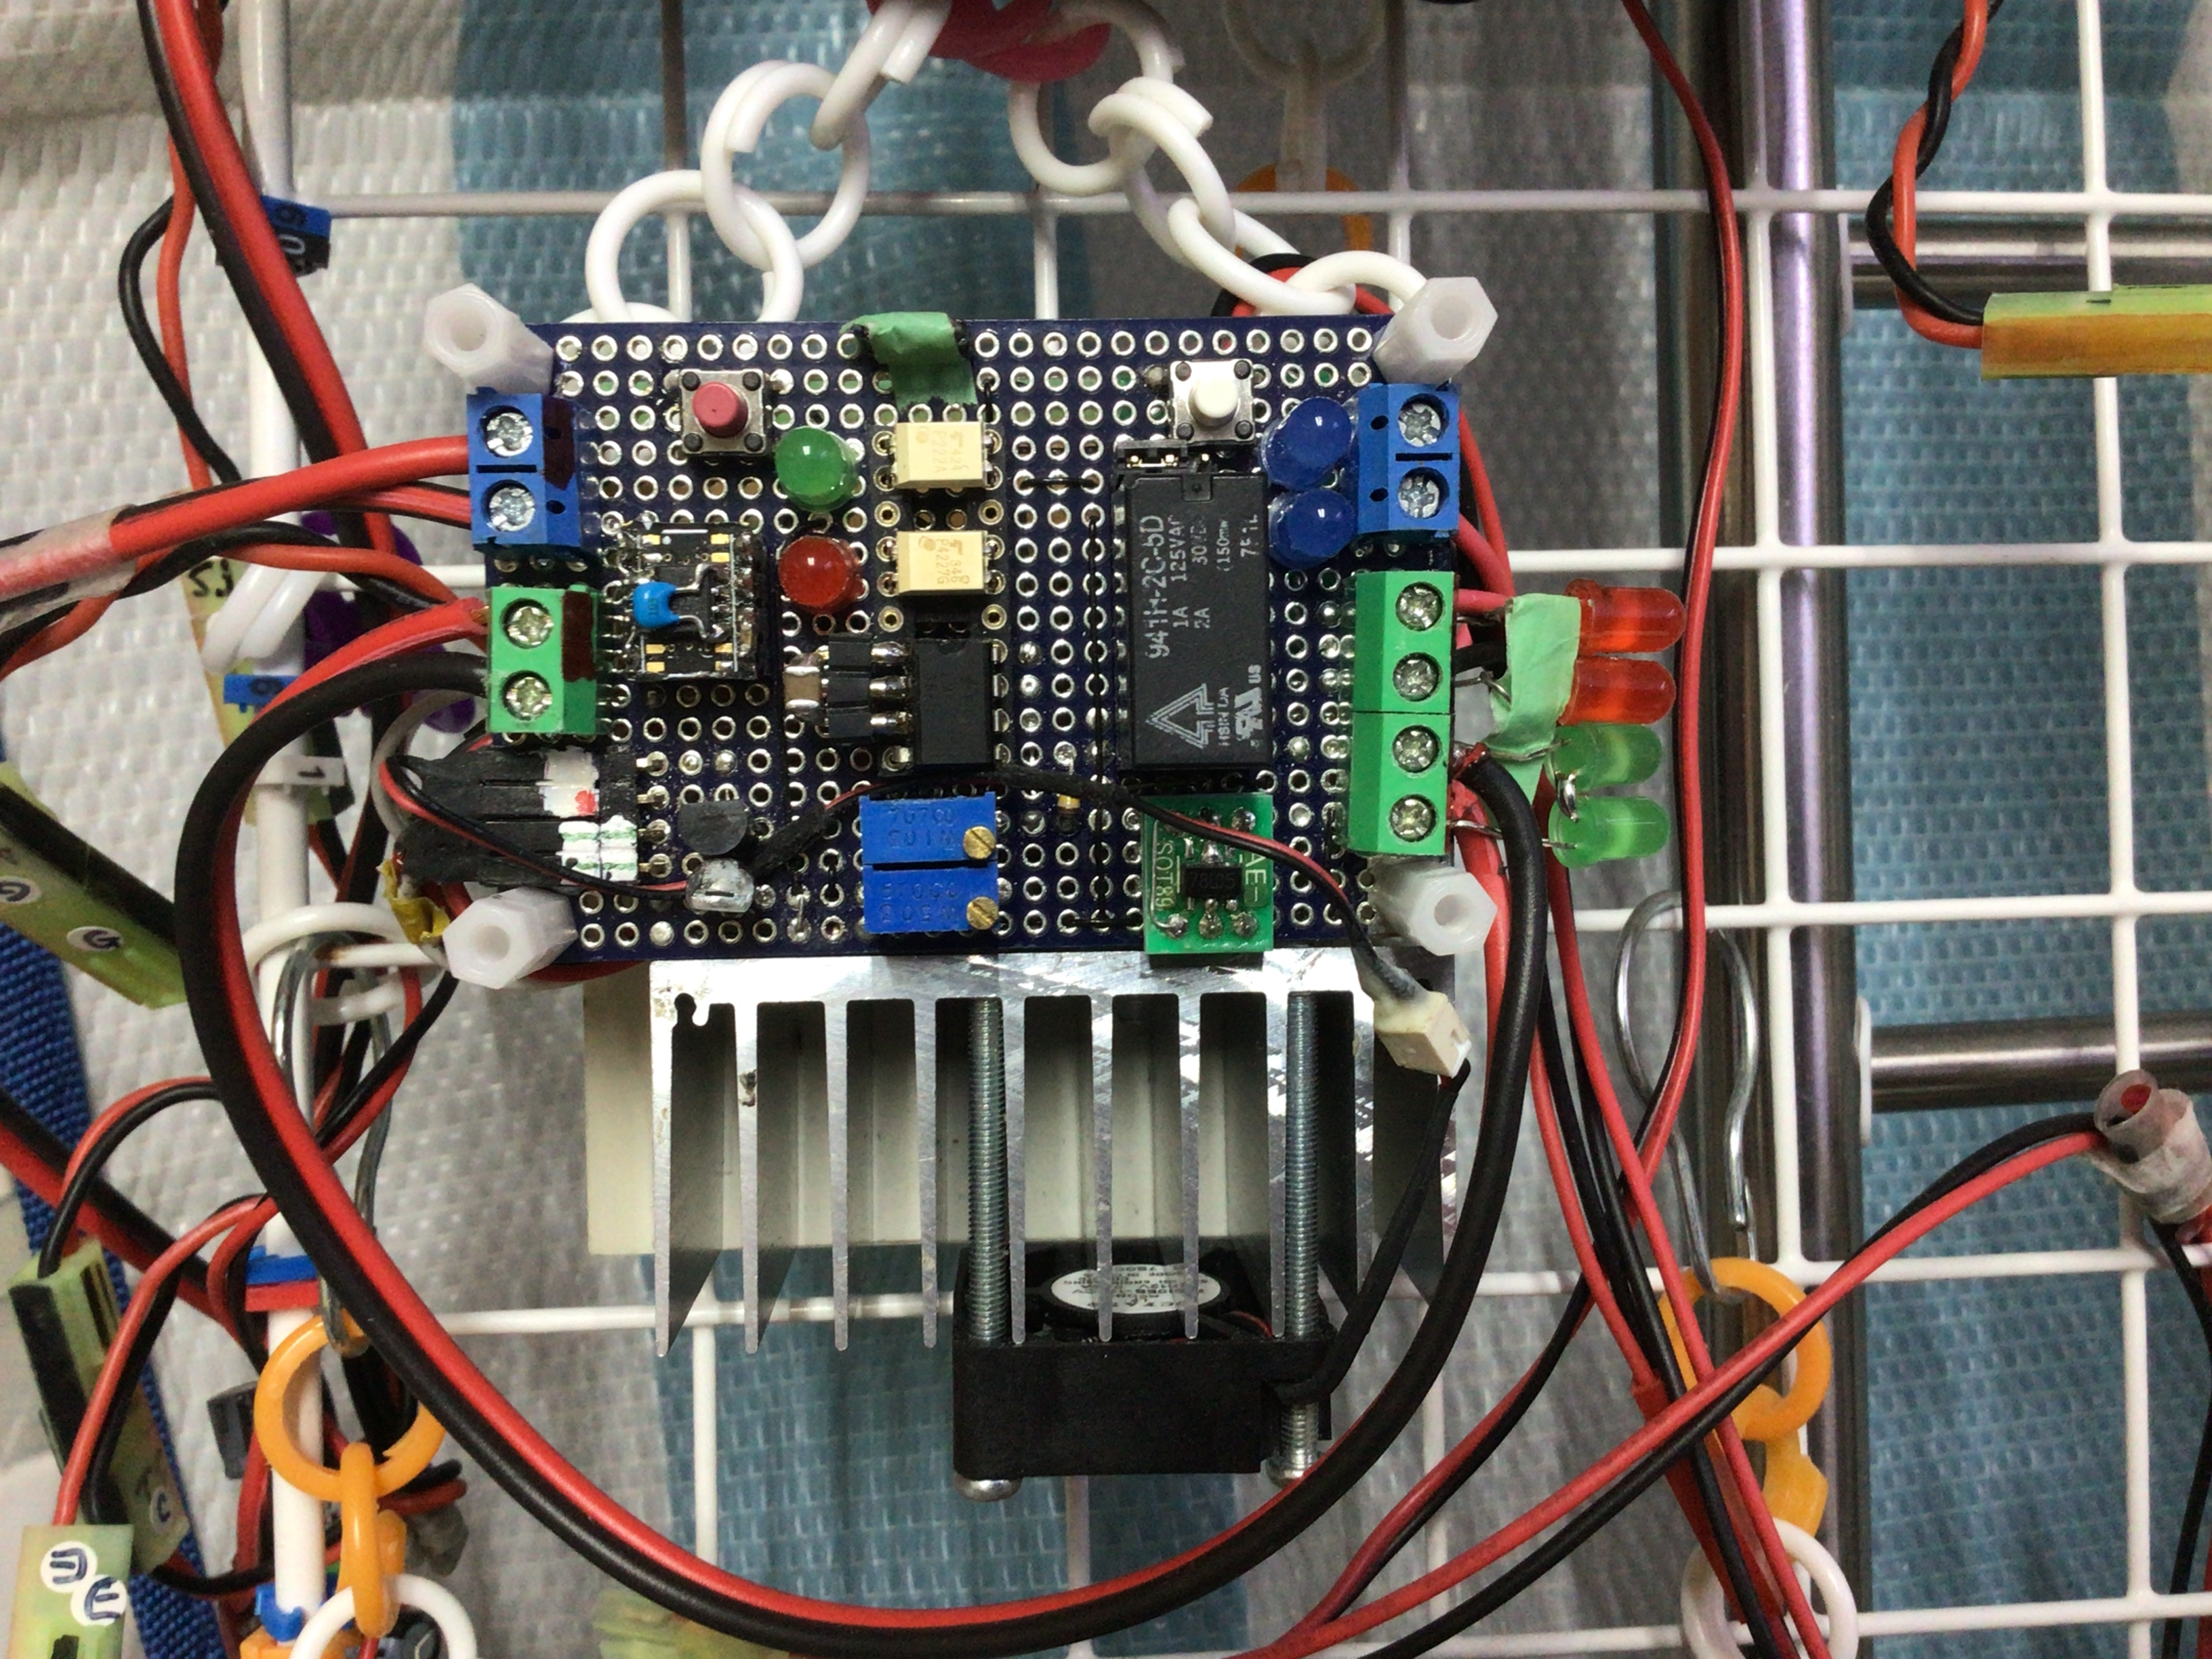
\includegraphics[width=7.5cm]{figspics/RaspberryComPoTE_figY.png}
\caption{電源供給・例外状態送出系の例}
\label{hohno:RaspberryComPoTE-Po1}
\end{figure}
\vspace{-1zh}
%%x%%

各IoTデバイス側に用意する昇降圧型のレギュレータには,4.5〜18Vの入力電圧を許容する3W級絶縁型昇降圧型DC-DCコンバータの MCWI03-12S05\cite{data:MCWI03-12S05}を採用し,最終的には安定した DC5V 最大600mA 供給している.
さらに,各IoTデバイスには,電源電圧変化の検出に特化した専用ICの M51957B(RNA51957B)\cite{data:M51957B}を配置し,次項で述べる例外状態を検出可能にした.

%% http://www.ti.com/lit/ds/symlink/lm338.pdf

%% ,一次側はDC16.5V,二次側はDC13.5V(通常時)または9V(例外状態通知時)とした


%% (※メモ:図)ここに電源出力系と各IoTデバイス側の受電系の図(図\ref{hohno:Po1})を入れる

%% (※メモ)過電圧遮断系も実装した

電源供給系の実装にあたっては,付加機能として設定以上の電流を検出した際に直ちに給電を停止し,音と光で警報を発報する機能も用意した.

シリーズ方式かスイッチング方式かによらず定電圧電源装置の多くは規定値以上電流が流れ続けた場合には一時的に給電を停止するか供給電圧を大きく下げ,過電流状態が除去されると元の電圧での給電を再開する機能を持つ.
{\tt Raspberry\-Com*PoTE}においても,最終的には長時間無停止無人運転を行うのでこのような機能は必要となるが,この機能が働く電流値は多くの場合装置ごとに決まっていて任意の電流値には設定できない.
さらに,{\tt Raspberry\-Com*PoTE}は現在も開発中のため試行錯誤を伴う運用がある.このような状況で,あらかじめ決めた以上の電流が意図せず流れた場合には,給電を直ちに完全に停止するとともに
光と音で警報を発するなどして開発者に知らせ,原因を除去するまでは自動での通電再開はできないようにする機能があるのが望ましい.

この機構を望んだのは,意図せぬ誤接続誤接触で電源系がショートしたのにそれが短時間だったため直ちに通電が回復してしまい,同じことが何度も発生しているのに異常と判断するのに時間を要した経験をしたためである.
{\tt Raspberry\-Com*PoTE}においては,4芯ケーブルが長くなるとケーブルの抵抗成分が無視できない大きさになり,引き回しによっては1Ωを超えることがある.このような場合,IoTデバイス側で電源まわりがショートしても非安定電源側ではたかだか5-10A程度の電流に留まってしまう.
このような場合,レギュレータの保護回路が働くまでに数10秒の時間を要したり,発熱はしてもは保護回路は全く働かず給電を続けたりする.
つまり,過電流検出と電流制限をレギュレータの機能に任せてしまうと,レギュレータの規定値を上回る電流を流さない限り保護回路は働かない上,多くの場合でケーブルの直流抵抗成分が供給上限以下の電流に留めてしまう.
例えば,今回用いた LM338 は,データシートによれば8A以上の電流が一定時間(過渡的には12A以上)流れないと保護回路が働かない.
一方,開発中のIoTデバイスに誤電流が流れた場合,1Aかそれ以下の電流が流れても異常状態ということがあり得る.
上述の理由により1A程度の電流はLM338にとっては正常の範囲であって過電流ではないので保護回路は働かないが,任意の値に設定できる過電流検出回路とそれに連携した給電停止回路を用意することで,異常状態検出機能とレギュレータの給電限界とを切り離して対応できる.
加えて,給電停止となったら音と光で警報を発する機能を用意すれば,原因を除去するまでは給電停止と警報の発報が繰り返され,
不用意な通電継続による回路の損傷を回避できる.


%%x%% この回路の概要を図\ref{hohno:RaspberryComPoTE-Po2}に示す.
%%x%%
%%x%% \vspace{-1zh}
%%x%% \begin{figure}[H]
%%x%% \centering
%%x%% 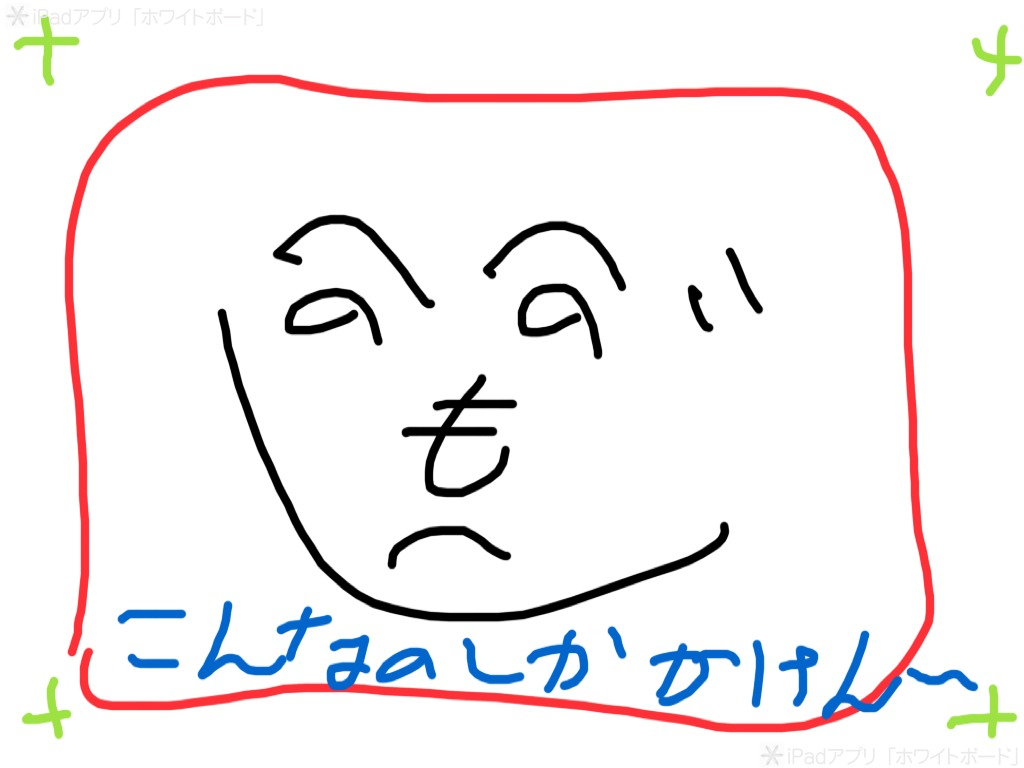
\includegraphics[width=5cm]{figspics/henoheno.jpeg}
%%x%% \caption{過電流検出・警報}
%%x%% \label{hohno:RaspberryComPoTE-Po2}
%%x%% \end{figure}
%%x%% \vspace{-1zh}
%%x%%
%%x%% %% 開発完了後の無停止運用においてはこのような手動操作を要求する機能は好ましくないが,開発完了まではこの機能を生かしておくことにした.

%% - - - - - - - - - - - - - - - - - - - - - - - - - - - - -

\subsubsection{例外状態検出系}
%% \vspace{-0.5zh}


すでに言及したように,
{\tt Raspberry\-Com*PoTE}では,接続したIoTデバイスを一斉に再起動したり,主としてハードウェア割り込みを発生させ「例外状態」の発生を通知する機能を持つ.
%% しくみを導入した.
%%  再起動(ハードウェア・リセット)やハードウェア割り込みの発生は,これらを受け入れる側にとっては例外的な状態であるため,これらを通知するしくみは「例外状態通知系」と呼んでいる.

%% {\tt Raspberry\-Com*PoTE}では,
現時点ではハードウェアリセット1種類とハードウェア割り込み1種類を提供しているが,これらの状態を通知するために上で述べた電源供給の非安定能を利用した.
例外状態の検出にあたっては,実装を簡単にするため,供給電圧が通常状態の約13.5Vから例外通知状態の約9Vへの降下を検出した時点でハードウェア割り込みを発生させ,それが一定時間(たとえば0.8秒)以上継続した場合にはさらにハードウェア・リセットを発生させる回路を用意した.
これにより電源電圧降下を2〜5Hzの速度で繰り返せばハードウェア割り込みは繰り返し発生し,ハードウェア割り込みハンドラ側でこの回数を数えることで,割り込み処理の挙動を順次変えることもできる.

現時点での例外状態検出系の実装を図\ref{hohno:RaspberryComPoTE-W}に示す.\\

\vspace{-1zh}
\begin{figure}[H]
\centering
%% 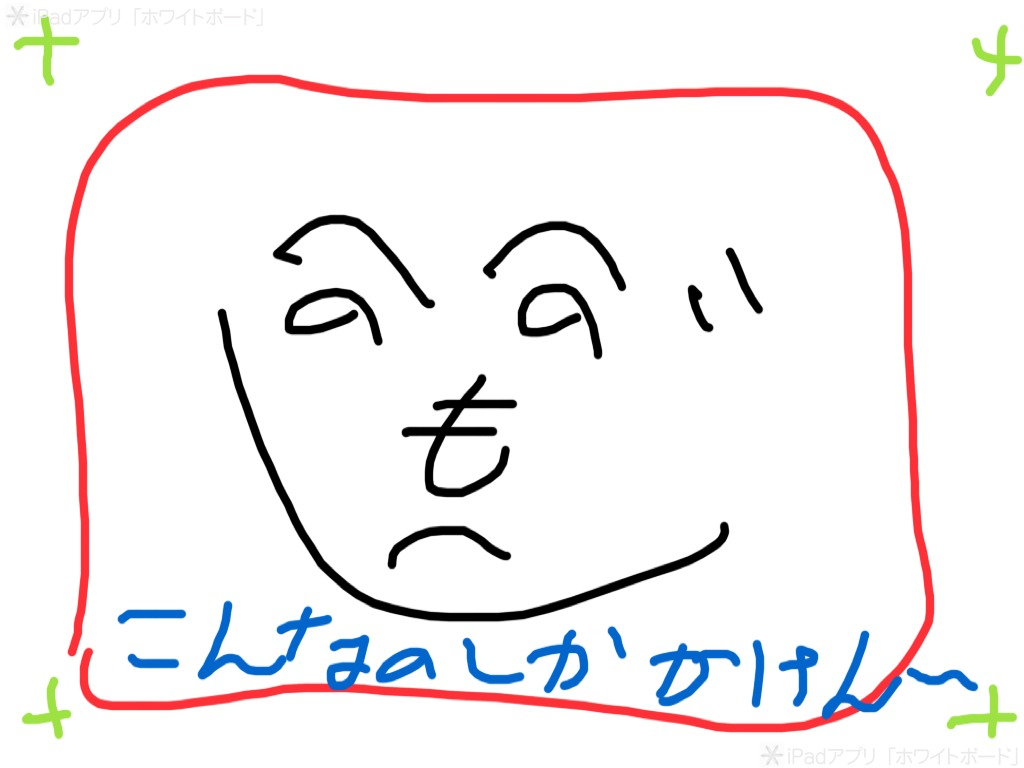
\includegraphics[width=5cm]{figspics/henoheno.jpeg}
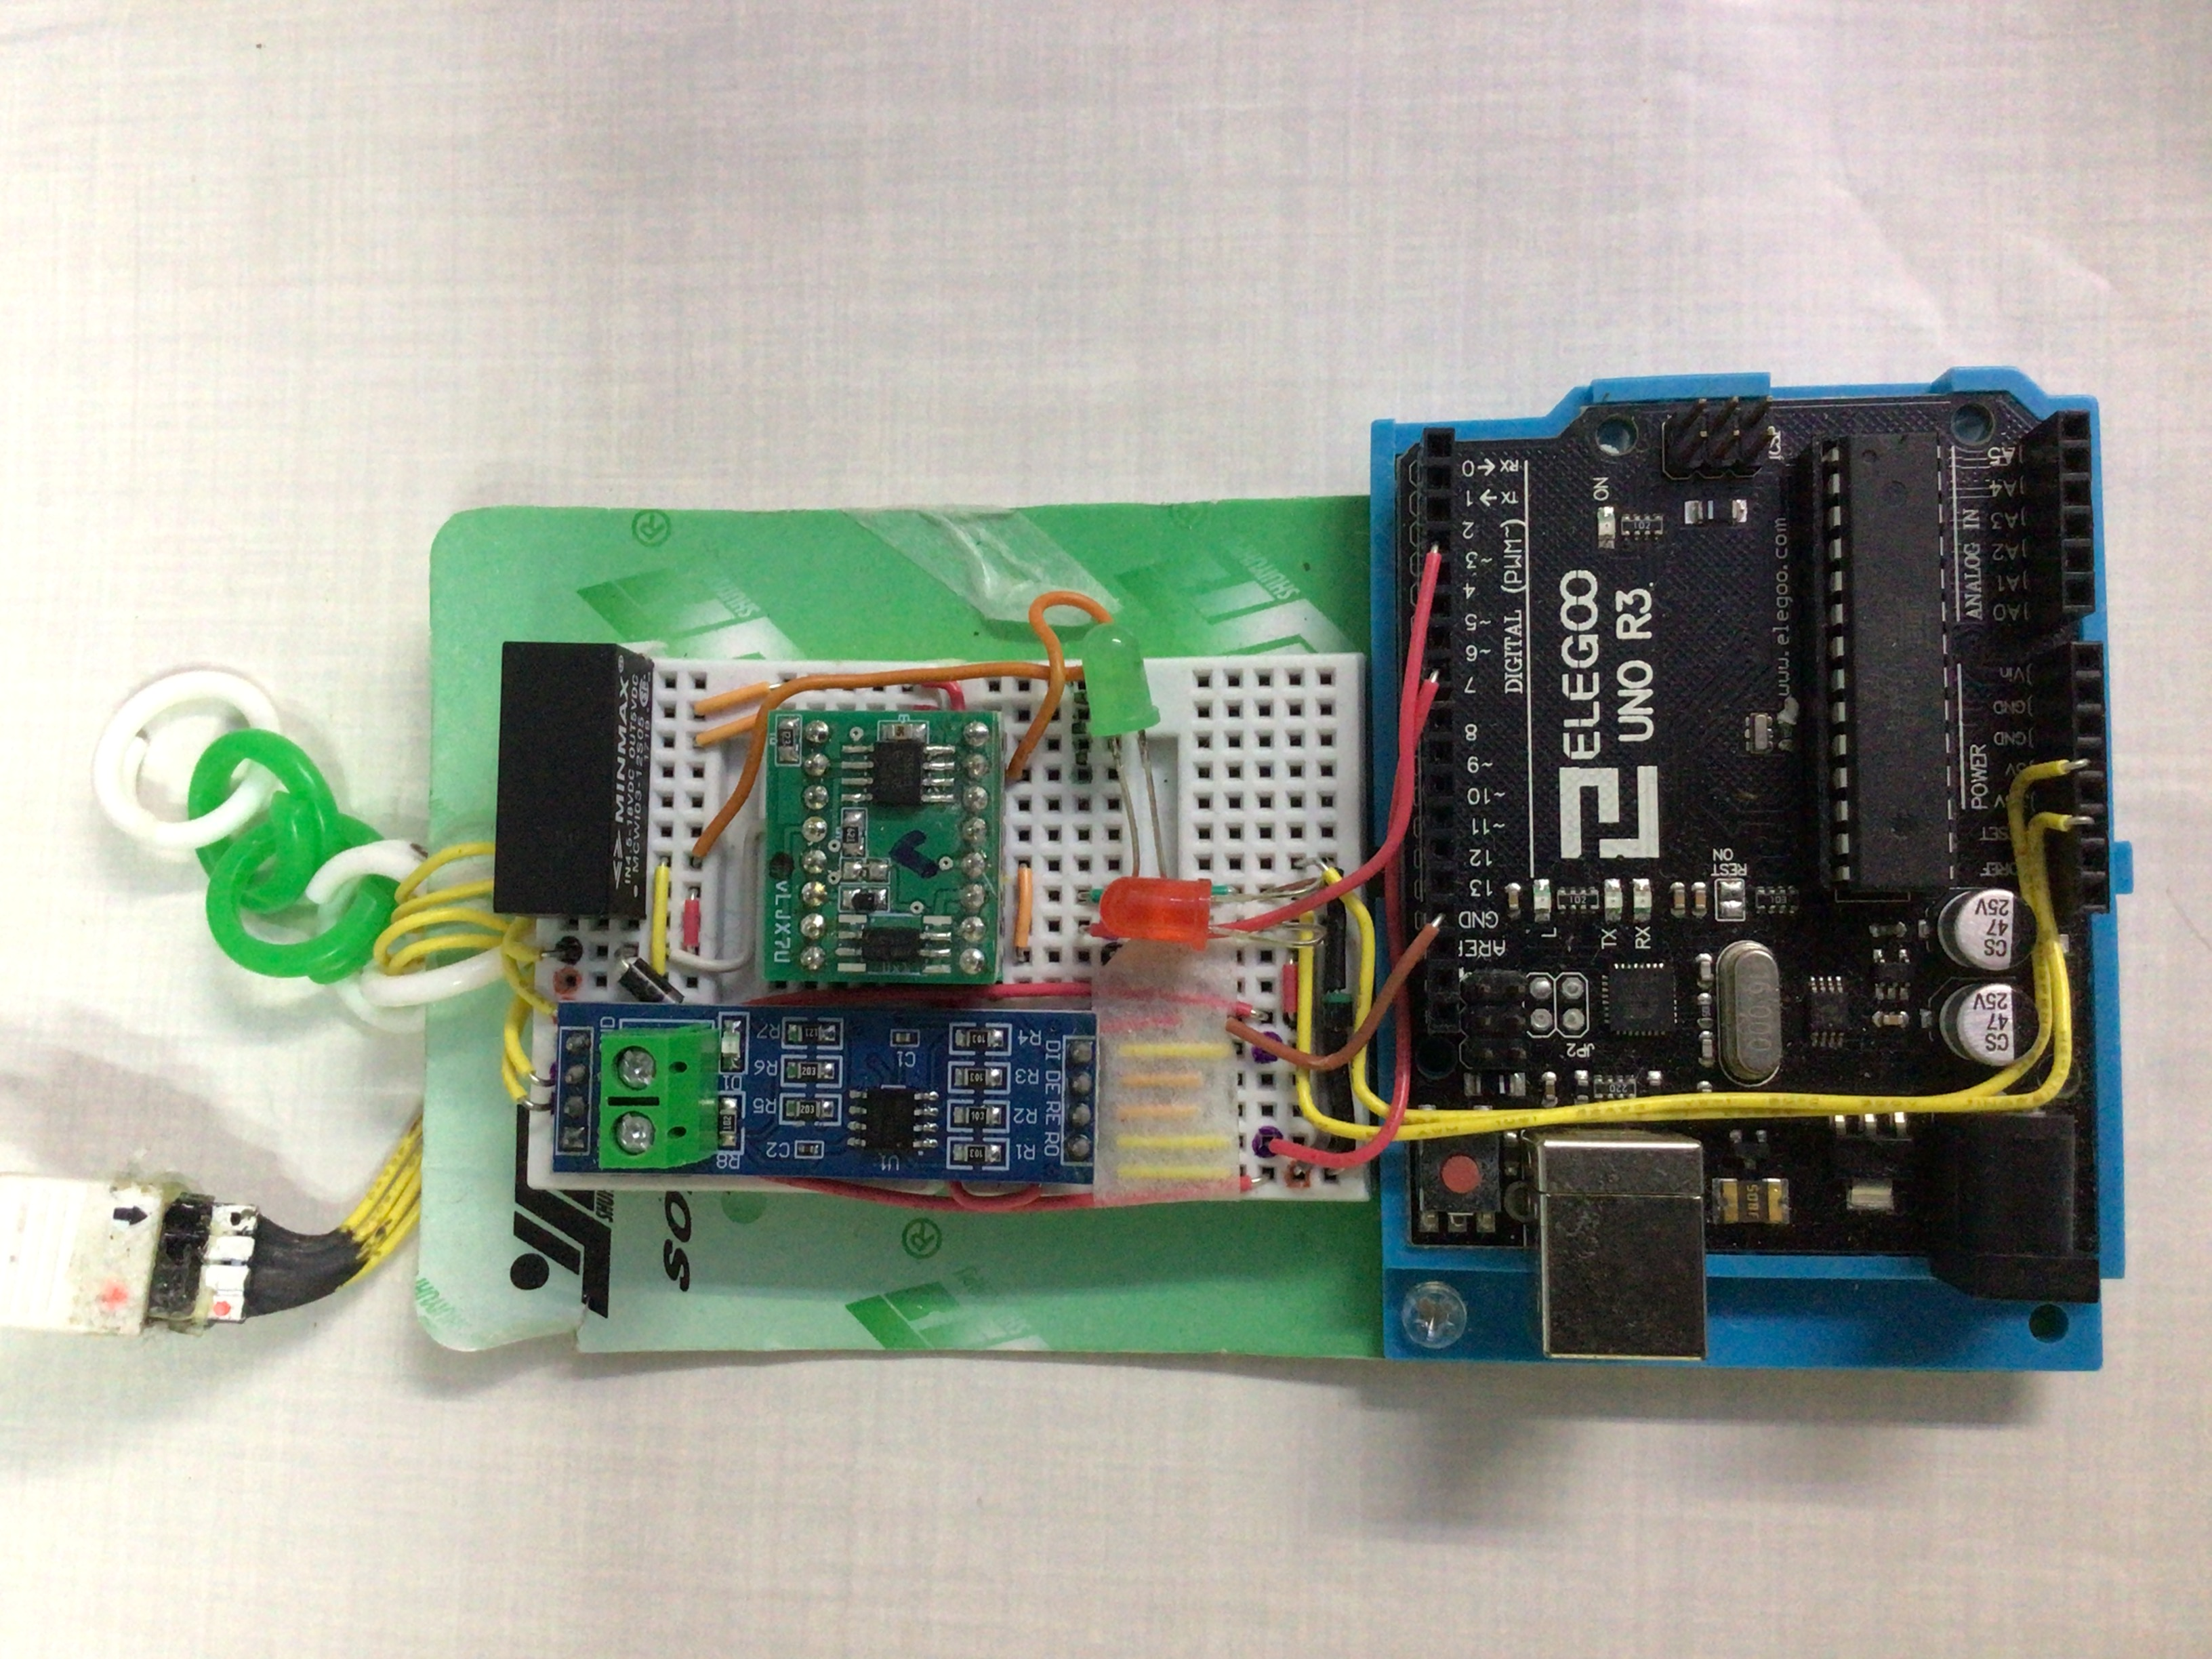
\includegraphics[width=8cm, angle=270]{figspics/RaspberryComPoTE_figW.png}
\caption{例外状態検出系の例}
\label{hohno:RaspberryComPoTE-W}
\end{figure}
\vspace{-1zh}
%%x%%
%%x%%(※メモ:図)ここにリセット・割り込み回路の図(ブロック図(と回路図?))(図\ref{hohno:RaspberryComPoTE-E})を入れる


%% - - - - - - - - - - - - - - - - - - - - - - - - - - - - -

\subsubsection{環境情報提供系}
%% \vspace{-0.5zh}


著者は,運用中のIoTデバイスの周囲の諸情報を環境情報と呼んでいる.
環境情報の筆頭は時刻情報である.時刻情報はIoTデバイスが何らかの情報を記録する際のタイムスタンプとなり,何らかの動作をする際のタイミングの基準となる.
時刻情報以外には気温や湿度を把握したい場合があるだろうし,用途によっては気圧や明るさ磁場電場なども取得できると好ましい.

これらの情報は,IoTデバイスによっては,デバイス自体が自ら取得して利用できる場合があるが,小型のIoTデバイスではそのような機構が省かれることもある.
たとえば,時刻であれば実時間時計(RTC - Real Time Clock)を搭載するだけでは正確な現在時刻を取得するには不十分である.
そのため時刻同期の仕組みが必要になるるが,パソコンでよく利用される NTPサーバへアクセスしてNTPプロトコルを用いて時刻同期をするには,IoTデバイス側にUDP/IPプロトコルスタックを用意し,IP到達性を確保するための物理層とデータリンク層を用意しなければならない.アドレス取得のための DHCPクライアントやアドレス解決のための DNS クライアント機能も必要になる場合もある.
IoTデバイスをできるだけ小規模に作ろうとした場合,NTPプロトコルによる時刻同期はソフトウェア領域を圧迫し新たなハードウェアの追加を必要とするなどオーバーヘッドが大きくなる.たとえば,Arduino UNO\cite{data:Arduino}を用いた計測系を作る場合,Arduino UNO のプログラム領域はわずか 30kB程度でありここにTCP/IPプロトコルスタックに加え,DHCP, DNS, NTP などのサービスを書き加えると30kBの領域の大半を消費してしまう.\\

%% (※メモ)引き続き書く

%%\vspace*{-1zh}
%%\subsubsubsection{環境情報提供サーバの時刻提供機能}

%% \vspace{0.5zh}
\noindent{\large{\textgt{\textbf{\underline{・環境情報提供サーバの時刻提供機能}}}}} \par
%% \vspace{0.5zh}

時刻情報の提供と取得は以下のように行う

まず時刻提供用の機材(環境情報サーバ)を用意する.必要なの以下の機能である.すなわちこの機材は上述の IoT デバイスと異なり時刻提供サービスへのIP到達性を持つ.なおカッコ内には必要とな具体的な機能である.

\begin{itemize}
\item NTPサーバに到達できる機能(TCP/IPプロトコルスタック,IP到達性.場合によってはIPアドレス取得機能と名前解決機能)
\item NTPサーバと時刻を同期を行い,内部のマイクロ秒カウンタの現在値とその時点でのUNIX秒(1970年1月1日0時0分0秒のUTCを0秒とする整数値)とのオフセットを求める機能(SNTPプロトコル)
\item RS-485回線に文字列を出力する機能(RS-485ドライバ)
\end{itemize}

この機能を使い,以下の手順で時刻情報をRS-485回線に送出する

\begin{enumerate}
\item 内部のマイクロ秒カウンタの下6桁がゼロになるタイミングの一定時間前(通常は100m秒程度)に改行文字を通信路上に送出(これが「予報」となる)
\item 内部のマイクロ秒カウンタの下6桁がゼロになるタイミングでプリアンブルとなる ``T'' を送出
\item 続いてこのタイミングにおけるUTC値を送出
\end{enumerate}

上記の機能を実現するため,現行の環境情報サーバは ESP-8266 を用い Arduino開発環境上で C++言語を用いて実装した(図\ref{hohno:RaspberryComPoTE-Z}).\\


\vspace{-1zh}
\begin{figure}[H]
\centering
%% 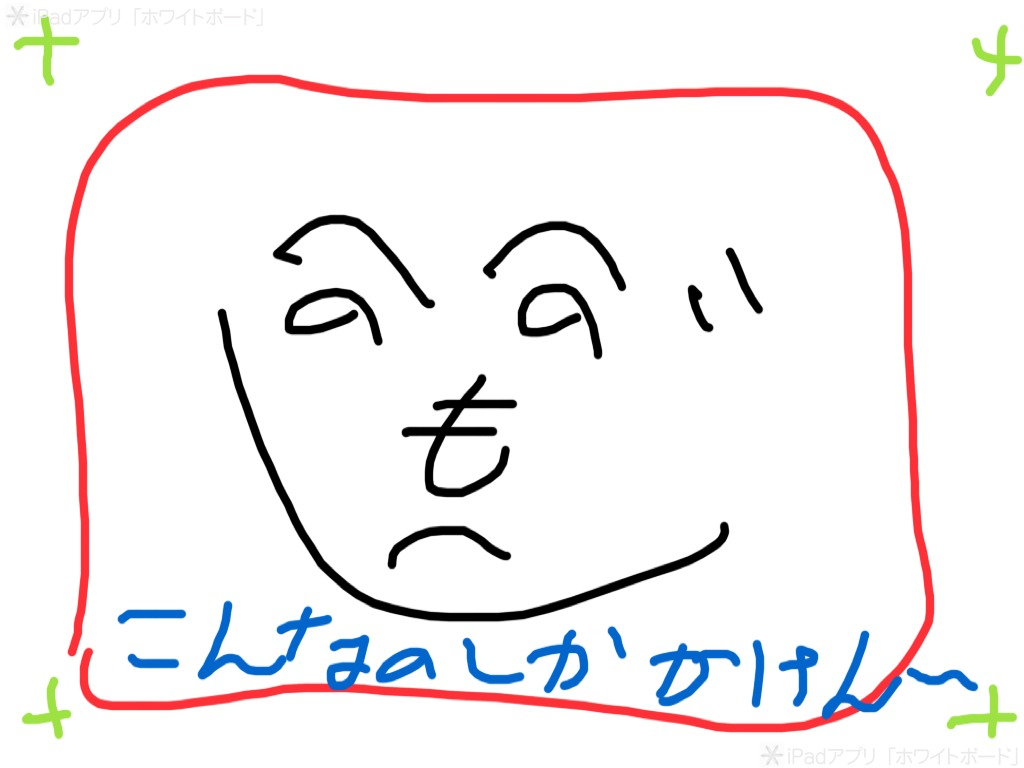
\includegraphics[width=5cm]{figspics/henoheno.jpeg}
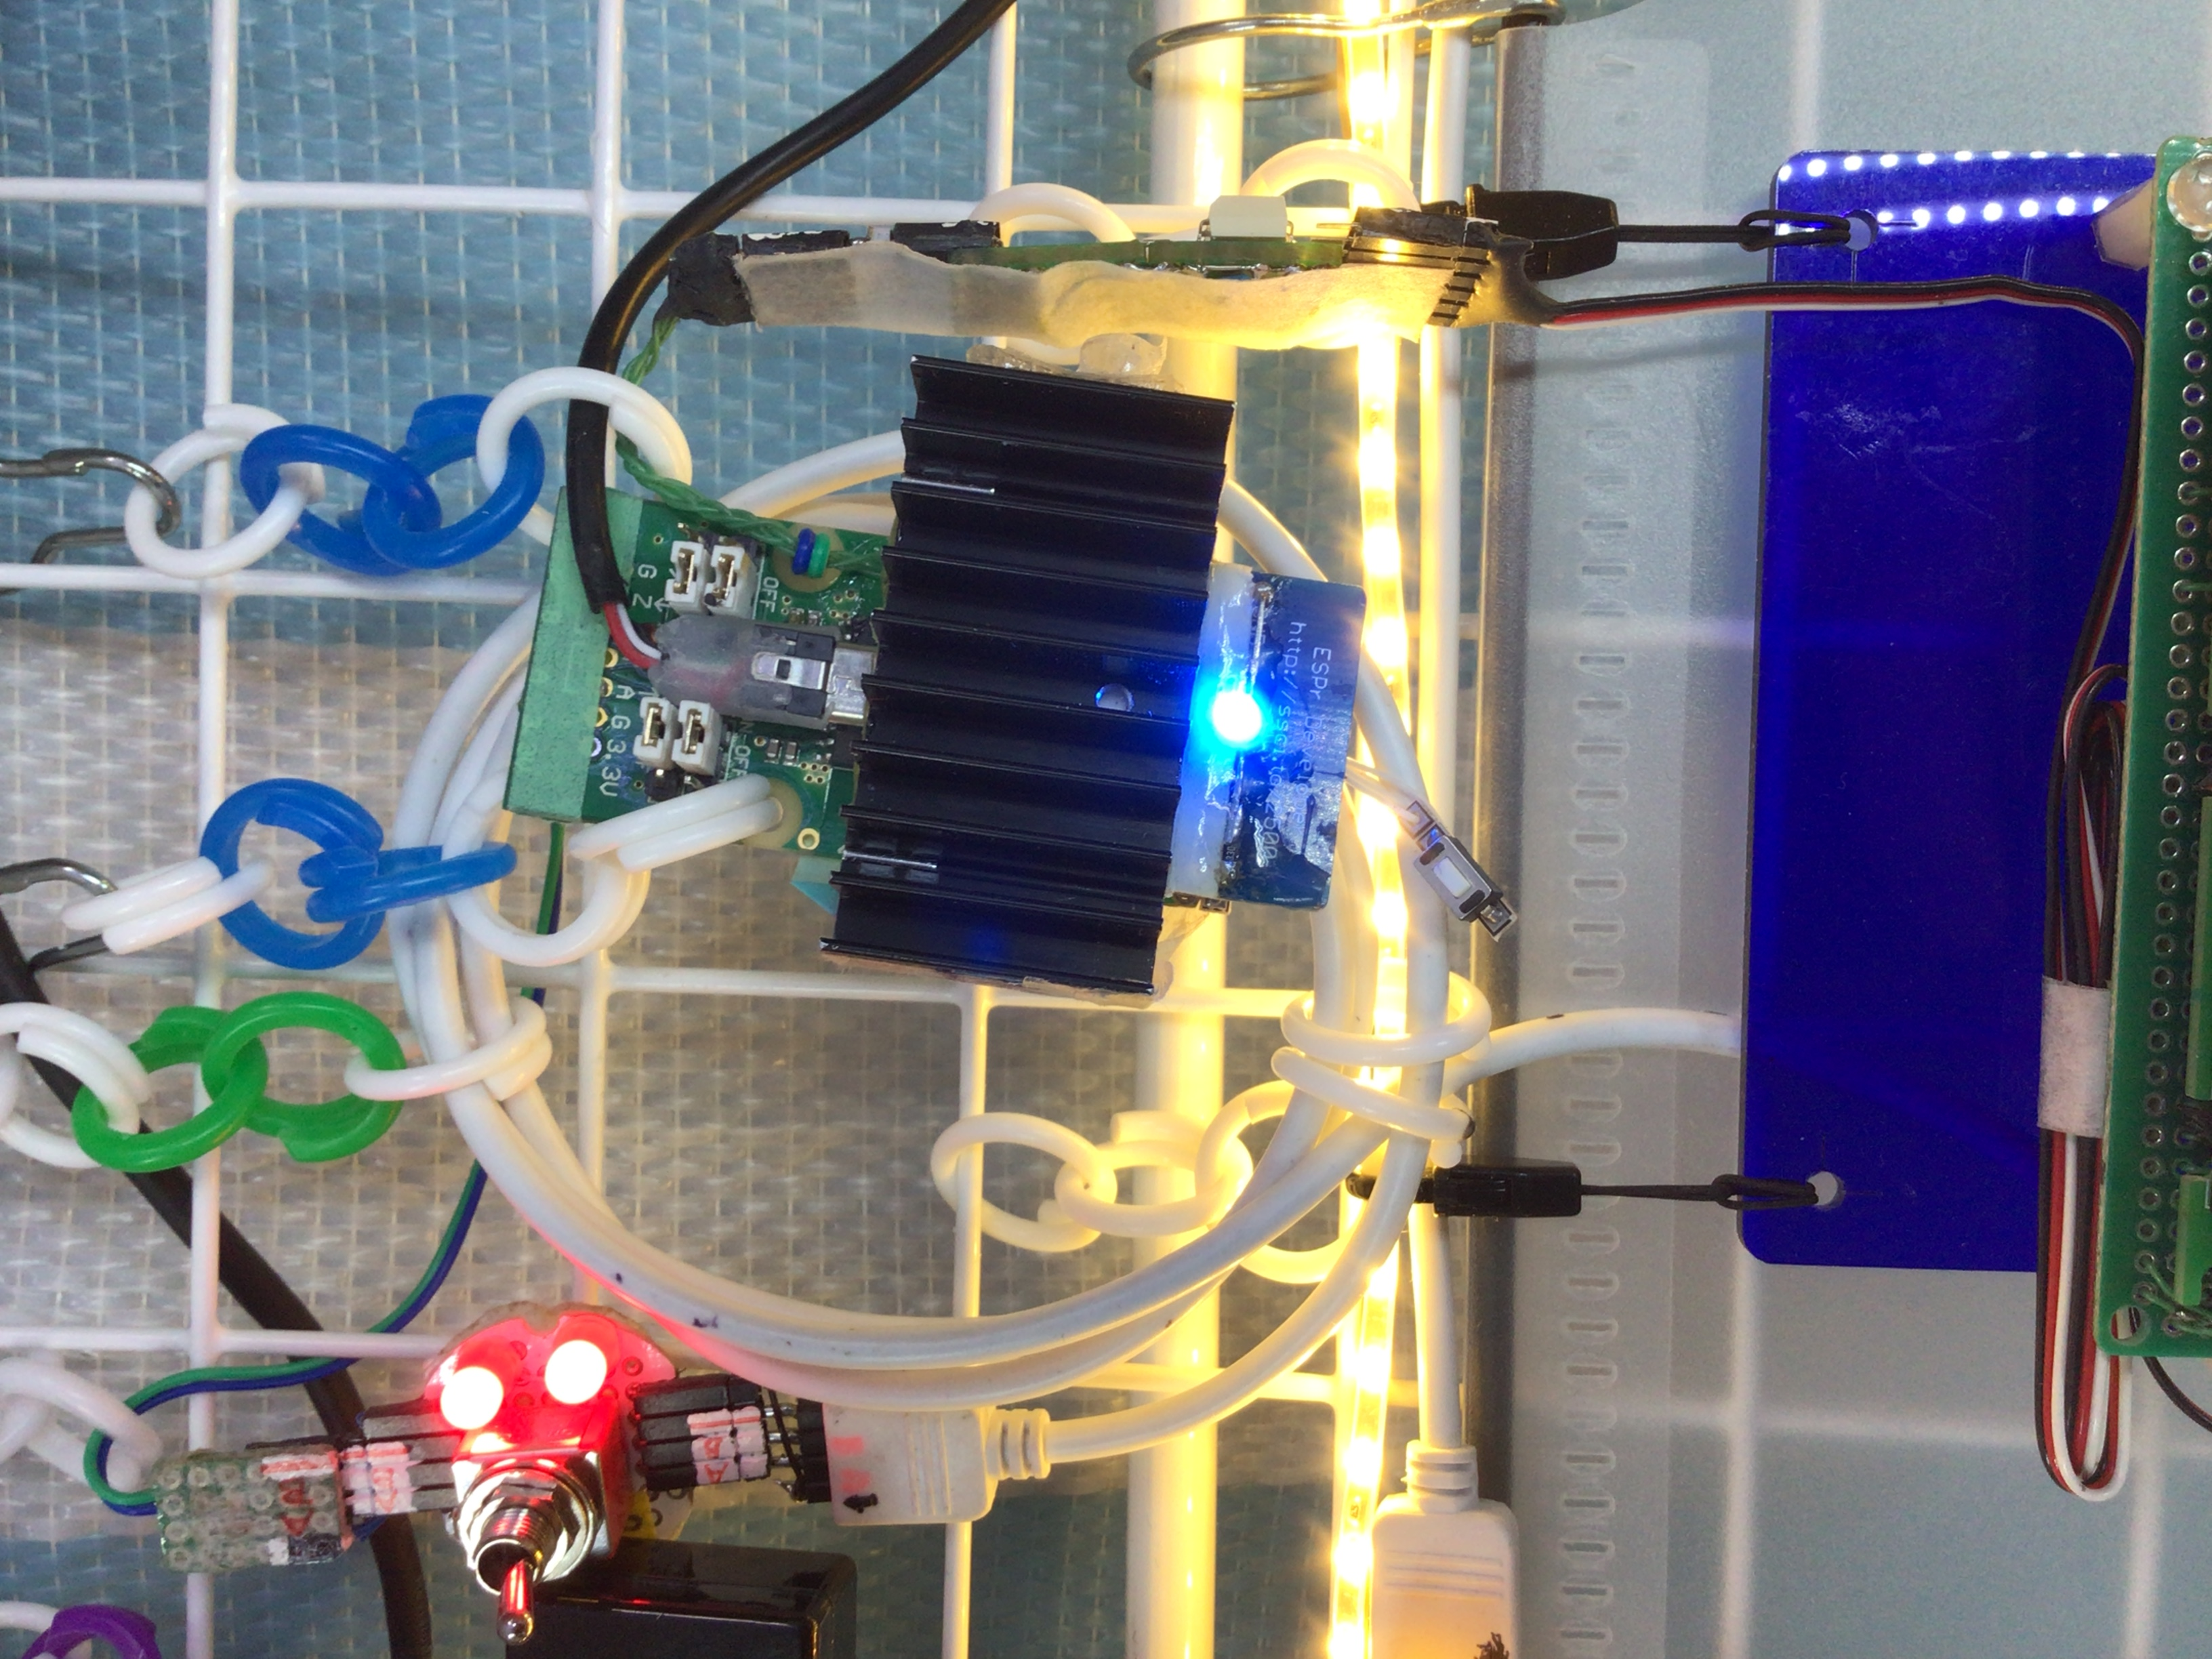
\includegraphics[width=8cm, angle=270]{figspics/RaspberryComPoTE_figZ.png}
\caption{環境情報提供系の例}
\label{hohno:RaspberryComPoTE-Z}
\end{figure}
\vspace{-1zh}
%%x%%
%%x%% (※メモ:図)環境情報サーバの構成(図\ref{hohno:RaspberryComPoTE-T})

%% \vspace{-1zh}
%% \subsubsubsection{環境情報提供サーバが提供する時刻との同期方法}

%% \vspace{0.5zh}
\noindent{\large{\textgt{\textbf{\underline{・環境情報提供サーバが提供する時刻との同期方法}}}}} \par
%% \vspace{0.5zh}

%% (※メモ)時刻情報の提供方法,受け取った側の同期方法

{\tt Raspberry\-Com*PoTE}を利用するIoTデバイスは RTCは搭載せずとも,Arduino UNOクラスの8ビットマイコンでも無理なく実現されている
「タイマ割り込みで更新するマイクロ秒カウンタ」が必須となる.そして以下の手順で,自らのマイクロ秒カウンタとUTCとのオフセットを決定する.

\begin{enumerate}
\item UARTから1バイト以上の読み出しが可能かを確認する.読み出せる文字がなければ他の作業に制御を移す.
\item もし1バイト以上の読み出しが可能なら1バイトずつ読み出し改行文字が現れるまで読み飛ばす.
\item 全て読んでも改行文字が現れなければ 1 に戻る
\item 改行文字が得られたら,一定時間以内(通常は10〜100m秒程度)に次の文字が届き,かつそれがプリアンブル(文字''T'')であることを期待してビジーループで待機
\item 1バイ以上の呼び出しが可能になったらその時点でのマイクロ秒タイムカウンタの値 T0 を取得
\item プリアンブルがこなければ T0 を破棄して 1 に戻る.
\item プリアンブル以後の文字を取得できるだけ取得してそれがUNIX秒として妥当な文字列なければ T0 を破棄して 1に戻る
\item UNIX秒として妥当な文字列が取得できたらこの文字列を UNIX秒を示す整数値に変換する.5で取得した T0は,このUNIX秒に対応するマイクロ秒カウンタの値である.
\end{enumerate}

この方法では,プリアンブルが到達した時点の内部カウンタの値とプリアンブルを送出した時点の UTC を得られるが,これをもって現在自国を決定する場合,時刻ずれを生じる要素として以下が考えられる.

\begin{enumerate}
\item 環境情報提供サーバのマイクロ秒カウンタから得られるUTCの推定値と実際のUTCのずれ(時刻情報提供サーバが保持するUTCの精度)
\item 環境情報提供サーバがプリアンブルを出力してから,IoTデバイスがUARTからプリアンブルを読み出すまでの時間
\item IoTデバイスが1文字読み出してからマイクロ秒カウンタの値 T0 を取得するまでの時間
\end{enumerate}

このうち 1 は NTP による時刻同期の精度であり,通常は1ミリ秒より十分小さな値で数〜数10マイクロ秒に追い込める場合が多い.
2は,RS-485回線の通信速度が {\tt Raspberry\-Com*PoTE} が採用する 57600bps の場合,140μ秒程度かかるが,ゆらぎのない固定値とみなせる値である.
3は,10マイクロ秒かそれより十分小さい以下であり,実験によってゆらぎのない固定値を取得可能である.
以上のことから {\tt Raspberry\-Com*PoTE} による時刻同期は1ミリ秒より十分小さい値に追い込める.

%%x%% %% \vspace{-1zh}
%%x%% %%% \subsubsubsection{{\tt Raspberry\-Com*PoTE}における時刻同期を実現するスケッチ}
%%x%%
%%x%% %% \vspace{0.5zh}
%%x%% \noindent{\large{\textgt{\textbf{\underline{・{\tt Raspberry\-Com*PoTE}における時刻同期を実現するスケッチ}}}} \par
%%x%% %% \vspace{0.5zh}
%%x%%
%%x%% 前目で述べた手順をArduino UNO用のクラスライブラリとして実装した.
%%x%%
%%x%% (※メモ)SoftwareSerial や Serial1 を使った
%%x%%
%%x%% (※メモ)どのくらいの大きさ?
%%x%%
%%x%% %% \vspace{-1zh}
%%x%% %% \subsubsubsection{時刻以外の環境情報の提供と利用}
%%x%%
%%x%% %% \vspace{0.5zh}
%%x%% \noindent{\large{\textgt{\textbf{\underline{・時刻以外の環境情報の提供と利用}}}}} \par
%%x%% %% \vspace{0.5zh}
%%x%%
%%x%%
%%x%% (※メモ)時刻以外の環境情報
%%x%%

%%x%% %% ---------------------------------------------------------
%%x%% %%  5. 評価(00%)0.75P / 6.25
%%x%% %% ---------------------------------------------------------
%%x%% \section{評価 \textcolor{red}{\small{\underline{(0.75p / 6.25)}}}}
%%x%% \vspace{-0.5zh}
%%x%% \label{sec:05evaluation}
%%x%%
%%x%% %% ---------------------------------------------------------
%%x%%
%%x%% \subsection{評価方法}
%%x%% \vspace{-0.5zh}
%%x%%
%%x%% (※メモ) 評価方法を提示する\\
%%x%%
%%x%% \subsubsection{電源供給系}
%%x%% \vspace{-0.5zh}
%%x%%
%%x%%
%%x%% (※メモ) 電源電圧の遷移が想定の速度でできるかを確認する\\
%%x%%
%%x%% %% - - - - - - - - - - - - - - - - - - - - - - - - - - - - -
%%x%%
%%x%% \subsubsection{例外状態通知系}
%%x%% \vspace{-0.5zh}
%%x%%
%%x%% (※メモ) 電源電圧の遷移によってハードウェア割り込みとハードウェア・リセットができるか確認する.ハードウェア割り込みが一定の速度で繰り返された場合,ハードウェア・リセットを起こすことなくハードウェア割り込みを繰り返せるかを確認する
%%x%%
%%x%% %% - - - - - - - - - - - - - - - - - - - - - - - - - - - - -
%%x%%
%%x%% \subsubsection{環境(時刻)情報提供系}
%%x%% \vspace{-0.5zh}
%%x%%
%%x%%
%%x%% (※メモ) 今回の評価は時刻同期に限定する. {\tt Raspberry\-Com*PoTE}にArduino UNOを接続して時刻同期させて上で毎正秒ごとに正秒パルスを発生させる.同時にGPS受信機からも正秒パルス出力し両者の時差をマイクロ秒単位で計測する
%%x%%
%%x%%
%%x%% %% ---------------------------------------------------------
%%x%%
%%x%% \subsection{評価結果}
%%x%% \vspace{-0.5zh}
%%x%%
%%x%% (※メモ) 評価結果を提示する\\
%%x%%
%%x%% \subsubsection{電源供給系}
%%x%% \vspace{-0.5zh}
%%x%%
%%x%% \vspace{-1zh}
%%x%% \begin{figure}[H]
%%x%% \centering
%%x%% 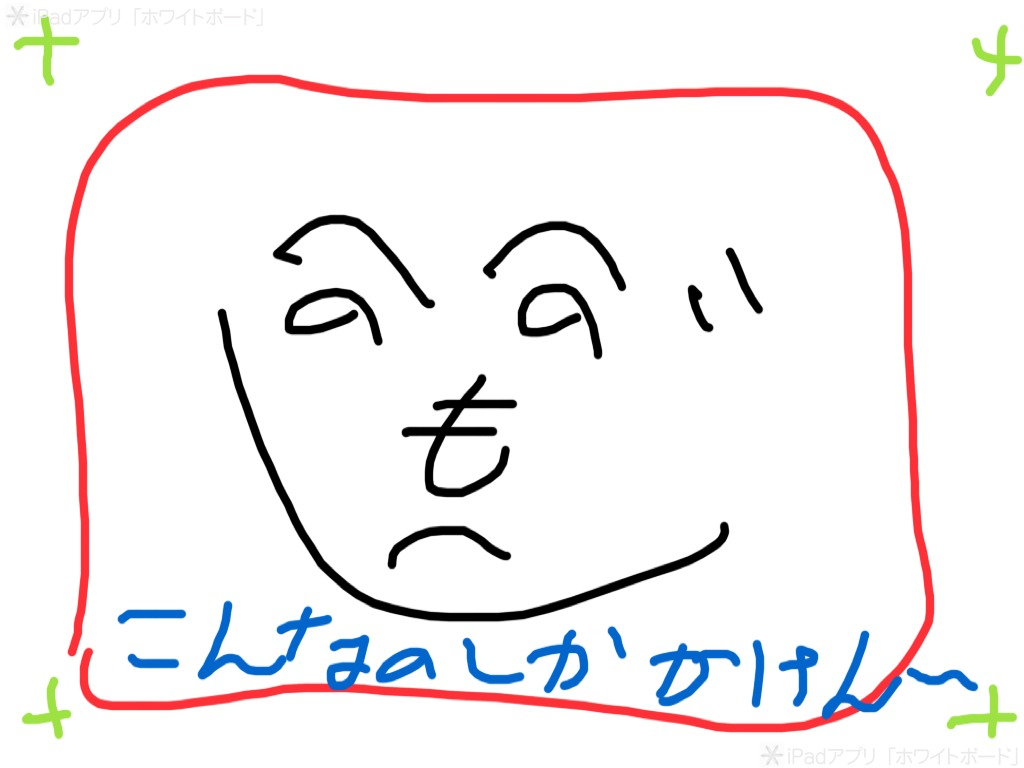
\includegraphics[width=5cm]{figspics/henoheno.jpeg}
%%x%% \caption{評価:電源供給系}
%%x%% \label{hohno:Eval-RaspberryComPoTE-Po}
%%x%% \end{figure}
%%x%% \vspace{-1zh}
%%x%%
%%x%% %% - - - - - - - - - - - - - - - - - - - - - - - - - - - - -
%%x%%
%%x%% \subsubsection{例外状態通知系}
%%x%% \vspace{-0.5zh}
%%x%%
%%x%% \vspace{-1zh}
%%x%% \begin{figure}[H]
%%x%% \centering
%%x%% 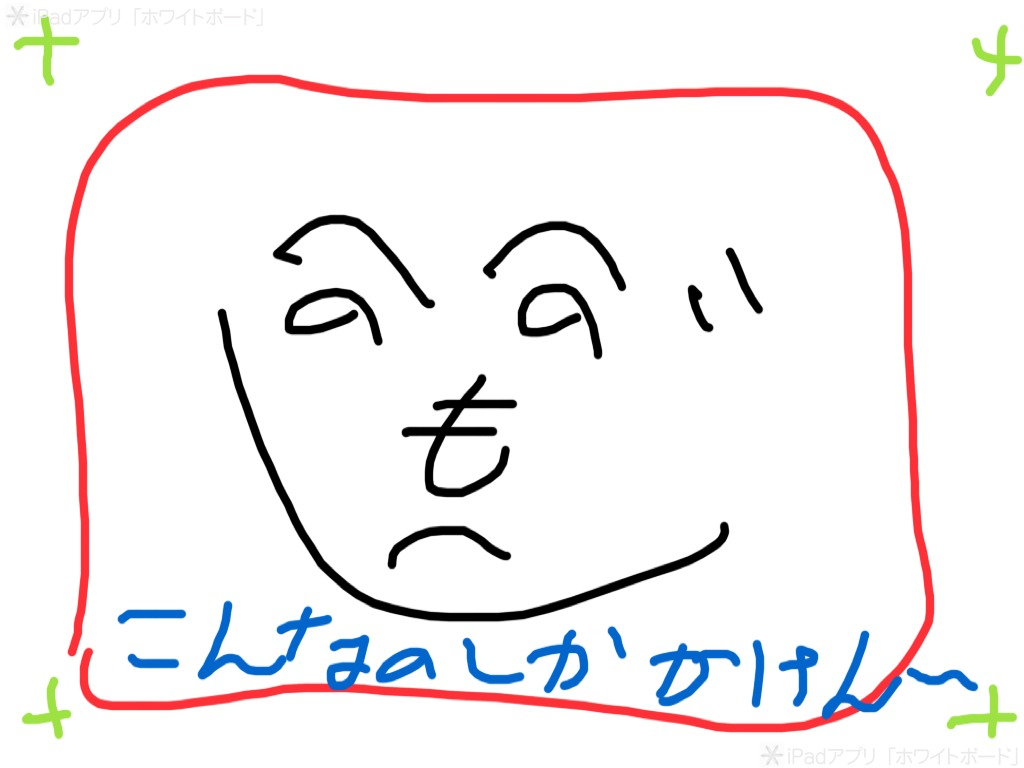
\includegraphics[width=5cm]{figspics/henoheno.jpeg}
%%x%% \caption{評価:例外状態通知系}
%%x%% \label{hohno:Eval-RaspberryComPoTE-E}
%%x%% \end{figure}
%%x%% \vspace{-1zh}
%%x%%
%%x%% %% - - - - - - - - - - - - - - - - - - - - - - - - - - - - -
%%x%%
%%x%% \subsubsection{環境(時刻)情報提供系}
%%x%% \vspace{-0.5zh}
%%x%%
%%x%% \vspace{-1zh}
%%x%% \begin{figure}[H]
%%x%% \centering
%%x%% 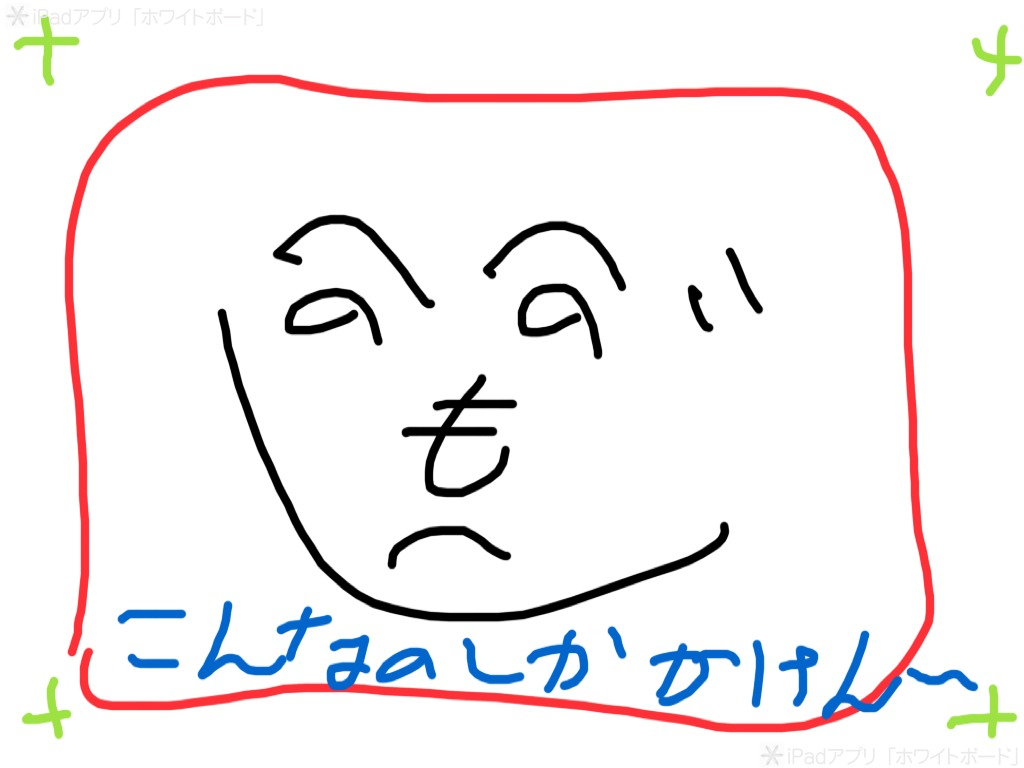
\includegraphics[width=5cm]{figspics/henoheno.jpeg}
%%x%% \caption{評価:環境(時刻)情報提供系}
%%x%% \label{hohno:Eval-RaspberryComPoTE-T}
%%x%% \end{figure}
%%x%% \vspace{-1zh}

%%x%% %% ---------------------------------------------------------
%%x%% %%  6. 考察(00%)0.75P / 7.0
%%x%% %% ---------------------------------------------------------
%%x%% \section{現状と今後 \small{\underline{(0.75p / 7.0)}}}
%%x%% \vspace{-0.5zh}
%%x%% \label{sec:06discussion}
%%x%%
%%x%% (※メモ) 他の方法との比較
%%x%% \\
%%x%%

%% ---------------------------------------------------------
%% 7. 今後の展開(00%)0.5P / 7.5
%% ---------------------------------------------------------

%% \section{現状と今後の展開 \small{\underline{(0.5p / 7.5)}}}
\section{現状と今後の展開}

%% \vspace{-0.5zh}
\label{sec:07nextstep}

著者は,{\tt Raspberry\-Com*PoTE} の一次試作の結果を元に,これを活用した IoTデバイス開発環境である {\tt Raspberry\-Workbench} を構成し,日々の IoTデバイスの開発を行なっている.
{\tt Raspberry\-Workbench} の有用性を定量評価するには{\tt Raspberry\-Workbench} を何式か用意して複数の被験者に既存の方法と比較させるなどの手順が必要であり,客観的な結論を得るにはまだ時間を要するが,著者は {\tt Raspberry\-Workbench}を日々利用する中で,{\tt Raspberry\-Workbench}は IoT デバイスの開発者に良好で快適な開発体験を提供するという印象を得ている.

{\tt Raspberry\-Workbench} の初期型は,2019年末頃から国内で開催されたものづくり愛好者のイベントで何度か図\ref{RaspberryWorkbench}のような動態展示を行った.
今回の DPSワークショップ2022 のポスター・デモセッションではこれに準じた動態展示を行う.

\begin{figure}[H]
\centering
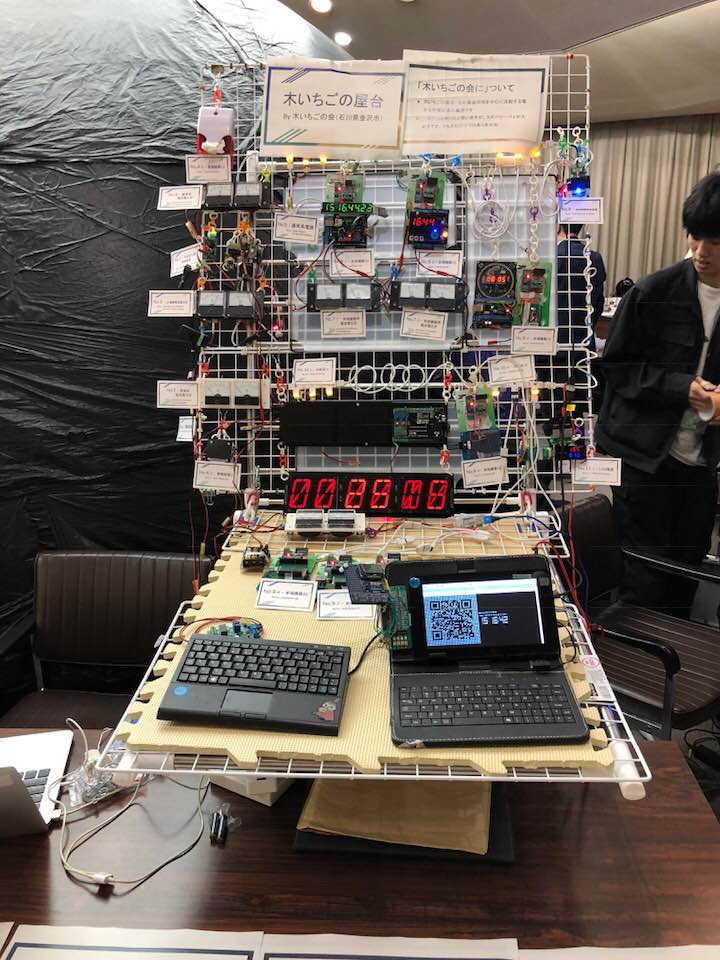
\includegraphics[width=6cm]{figspics/RaspberryWorkbench2.jpg}
\caption{ものづくりイベントにおける{RaspberryWorkbench}(2019年10月27日撮影)}
\label{RaspberryWorkbench}
\end{figure}

今後の展開については以下の3つの方向がある.

一つ目は,現在の {\tt Raspberry\-Com*PoTE} の量的拡張で,著者の研究室周辺で利用可能箇所を増やすとともに,著者の研究グループ内外への展開も行う.


二つ目は,現在の {\tt Raspberry\-Com*PoTE} の質的拡張で,距離と安定性を増したI2Cベースの近距有線ネットワーク機能の追加も検討している.また環境情報として時刻以外の供給を早期に開始する.


三つ目は,{\tt Raspberry\-Com*PoTE} の対応可能な環境の拡張で,現状より厳しい環境でも長期間に渡って安定に動作することを目指す,
具体的には,気温,湿度,気圧,振動などが現在の「室内」より厳しい自動車の車内(例えばキャンピングカーの居住部分等)への展開を目指す.



%% ---------------------------------------------------------
%% 8. おわりに(00%)(0.25P / 7.75
%% ---------------------------------------------------------

%% \section{おわりに \textcolor{red}{\small{\underline{(0.25p / 7.75)}}}}
\section{おわりに}
%% \vspace{-0.5zh}
\label{sec:07conclusion}

本報告では
多数のIoTデバイスに対し,外部から「電源」「時刻等の環境情報」さらに「例外状態の発生通知」を安定して提供するしくみを設計し,これを {\tt Raspberry\-Com*PoTE}(ラズベリー・コンポート)と名付け実装を行なった.
さらに,この方式を用いたIoTデバイス開発環境({\tt Raspberry\-Workbench})も試作し,日々の IoT デバイスの開発に投入している状況を報告した.


%% (※メモ)検討中

%% ---------------------------------------------------------
%%  謝辞(0%)(これ以降で 0.25p / 8.0)
%% ---------------------------------------------------------

%% \textcolor{red}{\underline{(※これ以降で 0.25p / 8.0)}}\\

%% \vspace{-0.5zh}
\begin{acknowledgment}

%%  \begin{spacing}{0.85}
%%    \small{
 本研究を遂行するにあたり,カナダ国ノバスコシア州立ダルハウジー大学コンピュータサイエンス学部教授の Prof. Sampalli および同教授の研究室の大学院生からは「ものグラミング」の有効性について検討する際に多くの示唆を得た.この経験が,{\tt Raspberry\-Com*PoTE}の開発を後押しした.
また,ユニバーサル・シェル・プログラミング研究所の當仲寛哲所長をはじめとする同社の研究部門の方々との議論も有益であった.ここに記して感謝したい.
%%    }
%%  \end{spacing}

\end{acknowledgment}


%% ---------------------------------------------------------

%% \newpage

%% \vspace{-0.5zh}
\begin{thebibliography}{2}

\bibitem{data:RaspberryPi}
  Raspberry Pi Foundation ``Rasberry Pi''
  \url{https://www.raspberrypi.org/}
  \refdatej{2022-08-26}


%% %% 01
%% \bibitem{hohno:monogramming1}
%%   大野,森,北口,中村,松浦,石山,當仲,ものづくりのための「ものグラミング」と実践的教育環境の構築,DICOMO2016,1335-1340, 2016-07.
%%
%% %% 02
%% \bibitem{misc:POSIXdocs1}
%%   What is POSIX?,The Open Group (オンライン),
%%   \urlj{https://collaboration.opengroup.org/external/pasc.org/plato/}
%%   \refdatej{2019-02-04}
%%
%% %% 03
%% \bibitem{matsuura:POSIXcentrics}
%%   松浦智之,大野浩之,當仲寛哲,ソフトウェアの高い互換性と長い持続性を目指すPOSIX中心主義プログラミング,デジタルプラクティス 8(4),352-360,2017-10-15.
%%
%% %% 04
%% \bibitem{misc:WSL_arch_overview}
%%   Seth Juarez,Windows Subsystem for Linux: Architectural Overview (オンライン),
%%   \urlj{https://channel9.msdn.com/Blogs/Seth-Juarez/Windows-Subsystem-for-Linux-Architectural-Overview}
%%   \refdatej{2019-05-22}
%%
%% %% 05
%% \bibitem{misc:firmata}
%%   Firmata Library
%%   \urlj{https://www.arduino.cc/en/Reference/Firmata}
%%   \refdatej{2019-05-22}
%%
%% 06
%% \bibitem{misc:kotoriotoko}
%%   秘密結社シェルショッカー日本支部,恐怖!小鳥男 (オンライン),
%%   \urlj{https://github.com/ShellShoccar-jpn/kotoriotoko}
%%   \refdatej{2019-02-04}

%% 07
\bibitem{hohno:RaspberryGate}
大野浩之,鈴木裕信,北口善明,
Raspberry Gateの設計と実装 : IoT時代に資するセキュリティゲートウェイの構築
電子情報通信学会技術研究報告,,
Vol.116, No.282, Pages 21-26
%% 08
\bibitem{hohno:RaspberryGuardian}
Shuting Hu, Hironobu Suzuki, Yoshiaki Kitaguchi, Hiroyuki Ohno, Srinivas Sampalli,
Design, Implementation and Performance Measurement of Raspberry Gate in the IoT Field,
Proceedings of the 2019 4th International Conference on Cloud Computing and Internet of Things, September 2019, Pages 82–89
DOI: 10.1145/3361821.3361827

%% 09
\bibitem{hohno:I2CwiredLAN-2017}
  大野浩之,データ通信機能に電源供給・回線復旧・基準信号供給機能を加えたI2Cベースの近距離有線ネットワークの提案,情報処理学会研究会報告,Vol.2017-IOT-38,No.12,2017-06-24.

%% 10
\bibitem{hohno:monogramming2}
  大野浩之,森祥寛,松浦智之,  ものグラミング2 --諸機能の選択と集中を徹底したPOSIX 中心主義に基づくIoT開発方式の提案--, 情報処理学会研究会報告,Vol.2019-IOT-46,No.00,2019-06-14.

\bibitem{misc:802.3cg}
  The New 10BASE-T1L Standard—Has Anything Changed?
  \url{https://www.analog.com/en/technical-articles/the-new-10base-t1l-standard.html}
  \refdatej{2022-09-20}

\bibitem{misc:DCC}
Digital Command Control
\url{https://en.wikipedia.org/wiki/Digital_Command_Control}
\refdatej{2022-08-26}

%% 以下要準備
%%
\bibitem{data:LM338}
  LM138 and LM338 5-Amp Adjustable Regulators
  \url{http://www.ti.com/lit/ds/symlink/lm338.pdf}
  \refdatej{2022-08-26}

%%
\bibitem{data:MCWI03-12S05}
  MINMAX MCWI03 series
  \url{https://www.cdiweb.com/datasheets/minmax/mcwi03-r2-110412.pdf}
  \refdatej{2022-08-26}
%%
\bibitem{data:M51957B}
  RNA51957A,B 電圧検出リセットシステムIC
  \url{https://www.renesas.com/us/ja/document/dst/rna51957ab-datasheet}
  \refdatej{2022-08-26}

%%
\bibitem{data:Arduino}
  Arduino Foundation ``Arduino''
  \url{https://www.arduino.cc/}
  \refdatej{2022-08-26}

%%
  %% \bibitem{data:B}
  %%   \urlj{https://}
  %%   \refdatej{2022-08-26}

\end{thebibliography}

%% ---------------------------------------------------------
